%\documentclass[conference]{IEEEtran}
\documentclass{article}
\usepackage{spconf}
\usepackage{amsmath,amssymb,amsfonts}
\usepackage{graphicx}
\usepackage{hyperref}
\usepackage{cite}
\usepackage{booktabs}
\usepackage{microtype}
\usepackage{url}
\usepackage{textcomp}
\usepackage{xcolor}
\usepackage{multirow}
\usepackage{siunitx}
\usepackage{placeins}
\usepackage{adjustbox}
%\usepackage{twemojis}
%\usepackage{emoji}

\usepackage[nolist]{acronym}
\begin{acronym}
\acro{stft}[STFT]{Short-Time Fourier Transform}
\acro{istft}[iSTFT]{Inverse Short-Time Fourier Transform}
\acro{tf}[T-F]{time-frequency}
\acro{fft}[FFT]{Fast Fourier Transform}
\acro{dft}[DFT]{Discrete Fourier Transform}
\acro{tfrs}[TFRs]{Time-Frequency Representations}
\acro{snr}[SNR]{Signal-to-Noise Ratio}
\acro{rir}[RIR]{room impulse response}
\acro{mse}[MSE]{mean-squared error}
\acro{rmse}[RMSE]{root-mean-squared error}
\end{acronym}

\newcommand{\kyung}[1]{\textcolor{magenta}{K: #1}}
\newcommand{\vesa}[1]{\textcolor{blue}{V: #1}}
\newcommand{\eloi}[1]{\textcolor{green}{E: #1}}
\newcommand{\shih}[1]{\textcolor{red}{S: #1}}
\newcommand{\nils}[1]{\textcolor{orange}{N: #1}}
% % Generated E5/E6 numbers; no E6 reference error.
\newcommand{\EfiveEDC}{9.513}
\newcommand{\EfiveC}{8.065}
\newcommand{\EfiveEDT}{0.487}
\newcommand{\EsixC}{0.717}
\newcommand{\EsixEDT}{0.0248}


\makeatletter
\g@addto@macro\small{%
  \setlength\abovedisplayskip{6pt plus 2pt minus 1pt}%
  \setlength\belowdisplayskip{6pt plus 2pt minus 1pt}%
  \setlength\abovedisplayshortskip{0pt plus 2pt}%
  \setlength\belowdisplayshortskip{2pt plus 2pt minus 1pt}}
\makeatother
\setlength\jot{2pt}

\renewcommand{\paragraph}[1]{\par\smallskip\noindent\textbf{#1}\hspace{0.5em}}

\begin{document}
\ninept

\title{Estimation of Room Impulse Responses from Handclaps}

\name{
%\begin{tabular}{@{}c@{}}
Shih-Yu Lai$^{1,2,3}$
\hspace{0.15em}
Kyung Yun Lee$^2$
\hspace{0.2em}
Nils Meyer-Kahlen$^2$
\hspace{0.2em}
Eloi Moliner$^2$
\hspace{0.2em}
Bing-Yu Chen$^1$
\hspace{0.2em}
Vesa Välimäki$^2$
%\end{tabular}
}


\address{
$^1$ National Taiwan University, Taipei, Taiwan \,
$^2$ Acoustics Lab, DICE, Aalto University, Espoo, Finland\\
$^3$ MoonShine Animation Studio, Taipei, Taiwan}

\maketitle
\begin{abstract}
Handclaps provide an equipment-free excitation for room acoustics, but their unknown and variable source waveforms make room impulse response (RIR) estimation difficult.
We introduce an anechoic handclap dataset containing 2,588 claps from
17 participants, designed to capture variability across natural claps and
different hand configurations.
%and study supervised estimation of a one-second RIR from a single reverberant clap. 
We first establish the performance attainable when the excitation clap is known using regularized deconvolution, and show that approximating the unknown excitation by cropping the direct sound from the reverberant recording is insufficient.
%Known-excitation inversion shows that the RIR is recoverable when the anechoic clap is available, whereas using the first 3 ms of the reverberant recording as an excitation estimate is insufficient.
We then study blind RIR estimation from reverberant handclaps, using the
anechoic handclap recordings to train a dedicated neural network with a
supervised regression objective. On the pooled measured-RIR benchmark, direct
regression improves normalized broadband energy-decay-curve error from
$-18.3$ to $-21.7$~dB and improves all other reported reconstruction metrics.
On phone-recorded handclaps, the inferred RIR spectra are more consistent across clap modes; because no paired reference RIR is available, this evaluation is qualitative.
These results establish a controlled single-clap RIR estimation framework and demonstrate its behavior on natural recordings.
\end{abstract}


\begin{keywords}Acoustic measurements, acoustic signal processing, deep learning, inverse problems, reverberation
\end{keywords}

\section{Introduction}

Measuring a \ac{rir} normally requires a known excitation signal reproduced through a loudspeaker at the measurement site.
Established methods, for example using swept-sine signals \cite{farina2000swept, prawda2022sweep}, provide accurate measurements but the required equipment and setup limit rapid or opportunistic measurements.
A handclap is a convenient alternative because it requires no playback hardware, is impulsive, and contains energy over a broad frequency range \cite{Seetharaman2012, papadakis2020handclap, devos2020improved, Fu2025,
halmrast2008simplified,huang2017impulse,rizzi2015rapid}.
Its spectrum, however, is not flat and depends strongly on hand configuration and execution \cite{repp1987sound,peltola2007synthesis,fletcher2013shock,jylha2008inferring}.
Previous work has therefore studied clap techniques, including gloves for improving measurement signal-to-noise ratio \cite{devos2020improved}.
Handclap responses can provide useful estimates of reverberation time and other energetic room-acoustic parameters \cite{Seetharaman2012, papadakis2020handclap}.


\begin{figure}[t]
    \centering
    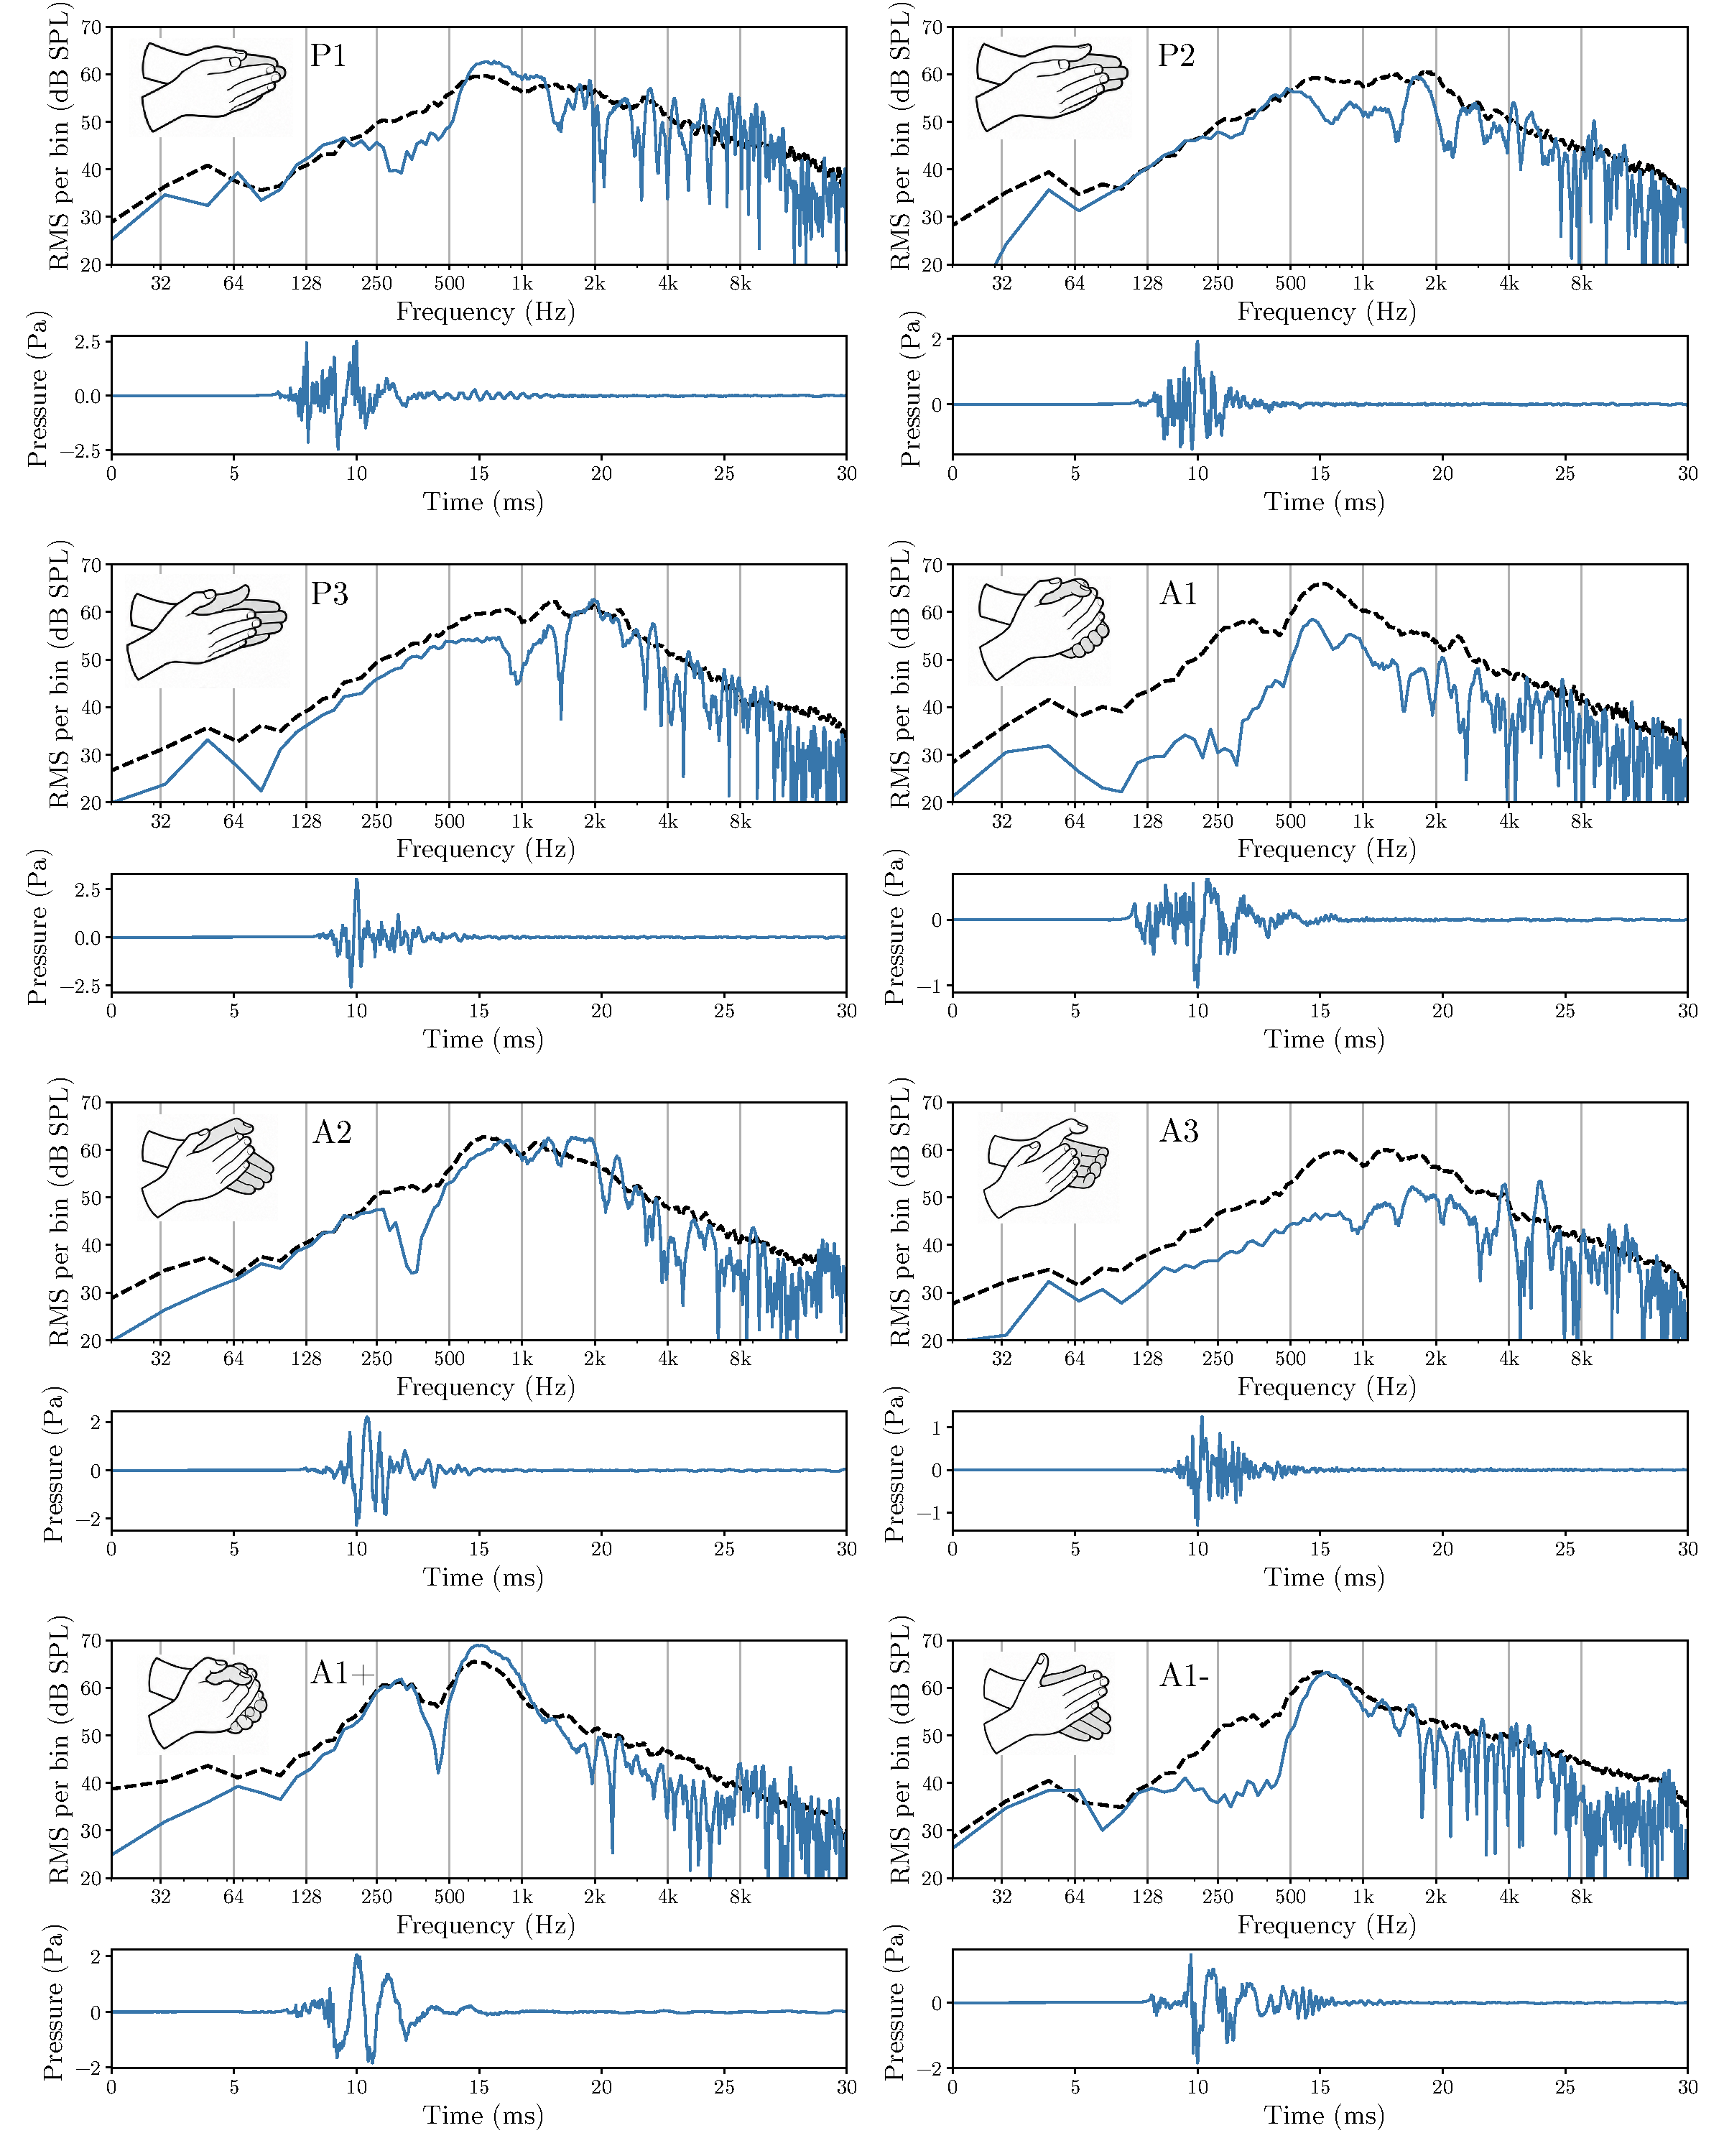
\includegraphics[width=\linewidth]{figures/clap_spectra_with_hands.pdf}
    \vspace{-0.8cm}
    \caption{Anechoic claps of different hand posture types. (Dashed line) Mean spectra over entire set of claps of that type. (Blue) one example spectra and corresponding time domain signal.}
    \label{fig:dataset}
    \vspace{-0.5cm}
\end{figure}

More recently, handclap recordings have also been used to approximate binaural RIRs and compared with time stretched pulse measurements \cite{nishimura2025binaural}. We study the more difficult problem of estimating the \ac{rir} itself from a single recorded handclap without knowing the excitation waveform.
% The observation contains both the clap and the room response, so excitation variation can be confounded with \ac{rir} structure.
%A handclap has an unknown, finite-duration waveform with its own spectral structure. 
The recorded signal is the result of convolving the impulse-excited \ac{rir} with a handclap, which entangles excitation-dependent and room-dependent features.

We address this problem using a newly recorded, anechoic handclap corpus that captures excitation variability and allows controlled training pairs to be constructed with known \acp{rir}.
In this contribution, we first introduce the anechoic handclap dataset (Sec.~\ref{sec:dataset}). Then, we quantify RIR recoverability when the true anechoic excitation handclap is known, using both unregularized and Tikhonov-regularized deconvolution.
We then test cropped-excitation baselines that use the first 3 or 6 ms of the
reverberant clap recording as an excitation estimate. Because this short-window approximation is inadequate, we propose estimating the \ac{rir} from the complete reverberant handclap using a two-stage time--frequency/time-domain neural network adapted from
\cite{moliner2026ambisonics} (Sec.~\ref{sec:problem}).




The controlled benchmark combines procedurally generated Shoebox responses with measured \acp{rir} from MIT ~\cite{mit}, BUT ~\cite{but}, ACE ~\cite{ace}, and OpenAIR ~\cite{OpenAIR} datasets. 
Across the pooled measured \acp{rir}, neural regression improves on both
cropped-excitation baselines for all reported acoustic, spectral, and waveform
errors. Finally, we examine qualitative real-world examples using phone recordings of eight handclap modes in seven rooms (selected two rooms as demos): a medium-size
meeting room and a highly reverberant hallway.
Within each room, the recorded spectra vary substantially across claps,
while the spectra of the inferred \acp{rir} are visibly more consistent
over much of the displayed frequency range (Sec.~\ref{sec:setup}). Code, demo website and datasets are here: \footnote{https://github.com/Akinesia112/ClapRIR.git}
\footnote{https://aaltoacousticslab.github.io/clapRIR-demo/}

Our contributions are:
\begin{itemize}
    \item an anechoic handclap corpus with 2,588 segmented events from 17 participants, covering natural handclaps and prescribed hand configurations;
    \item a controlled single-handclap RIR study comparing known-excitation
    inversion, 3- and 6-ms excitation approximations, and direct one-second neural regression; and    
    \item a qualitative real-world-recording experiment illustrating how
    handclap-dependent spectral variation is reduced through RIR estimation.
\end{itemize}




% This paper is organized as follows. Sec.~\ref{sec:dataset}... Sec.~\ref{sec:problem}... Sec.~\ref{sec:setup}... Sec.~\ref{sec:discussion}... Sec.~\ref{sec:conclusion}...

\section{Anechoic Handclap Dataset}
\label{sec:dataset}


We collected isolated handclaps in the large anechoic chamber ``Lampio'' at Aalto University.
In the course of the recording session, 17 participants were asked to take place in the center of a circular array of eight equiangularly spaced microphones with a radius of 2~m. Seven of these microphones were G.R.A.S. Type 46AF connected to a G.R.A.S. 12AG preamplifier. The microphone behind the listener belonged to a G.R.A.S. Type 40HF low noise measurement system. All microphones were gain adjusted after recording using a recording from a BK 4231 calibrator. 

At first, participants were prompted to ``clap as you normally would'' and ``clap as you would when trying to hear the sound of the room''. Then, they were shown a paper with picture of eight specific hand configurations from \cite{peltola2007synthesis}. Three positions labeled with ``P1''--``P3'' ask for holding both hands paralel, with decreasing overlap of the hands. The positions labeled with ``A1''--``A3'' follow the same logic, but ask for holding the hands at an angle.
For ``A1$+$'' asks for cupping the hand, and ``A1$-$'' for keeping the fingers straight. In each condition, participants were asked to clap 15 times. The protocol therefore requested 150 handclaps per participant. However, some participants missed a few claps, or clapped too often.

After recording, the files were segmented using a semi-automatic procedure. First, level peaks were identified. Then, claps whose maximal level was at least $-30$~dB below the strongest peak of the 15 claps of that participant and clap type were extracted; the extraction windows started 10~ms before, and ended 50~ms after each peak. Some spurious peaks were removed manually. All claps were visually examined. All in all, the corpus contains 2,588 eight-channel anechoic claps 
\footnote{The full dataset is available online, see \nils{Dataset Links}}
.

Figure~\ref{fig:dataset} shows average spectra per requested clap type, along with one example in time and frequency domain each. All claps show bandpass characateristics. As analyzed previously, the center frequency depends on the clap type \cite{peltola2007synthesis}. In addition, it can be seen that the examples contain some sharp spectral minima at high frequencies. Moreover, when analyzing the duration of each clap as the length between the times the the pressure crosses the $-60$~dB mark relative to the maximum pressure of the peak, median times of 4.85~ms for A3, to 6.46~ms for A1+, which is the cup clapped, are found.
%A deterministic quality screen retains 2,065 events from 15 participants and excludes 523.
%Of the excluded events, 417 belong to recording sessions whose detected handclap-run structure did not satisfy the acquisition
%protocol, and 106 belong to blocks whose segmentation brackets crossed item boundaries.
%No manual event-level screening is used.
For our experiments, claps from 12 participants were used for training and
3 were held out for testing; the remaining 2 participants were excluded
because their recording sessions did not satisfy the acquisition protocol
under the automatic quality-control procedure. For training, claps are further reduced to 20-ms support. Also, we used the samples from all clap types for our experiments. \footnote{Due to additional, automatic quality control, only 2065 claps were currently used for training.}

% Figure~\ref{fig:dataset-stats} summarizes retained-event counts, digital
% signal energy over the 20-ms training support, and the 5--95\% cumulative
% energy duration within that support. The energy values are uncalibrated
% digital quantities, and the support-limited duration is not the full clap
% duration.

%The recording protocol defines eight prescribed hand-configuration labels with different handclap poses
% : \shih{P1--P3, A1--A3, A1$-$, and A1$+$ }
%(\cite{repp1987sound, peltola2007synthesis}).
%These labels are also used in the phone recordings.
%The anechoic event metadata do not provide a verified mapping from individual retained events to these labels, so mode-specific anechoic statistics are not reported. 
%To construct controlled training pairs, retained anechoic handclaps are convolved with target RIRs according to \eqref{eq:forward}, producing reverberant observations with known target RIRs while preserving measured excitation variability.

% \begin{figure}[t]
%     \centering
%     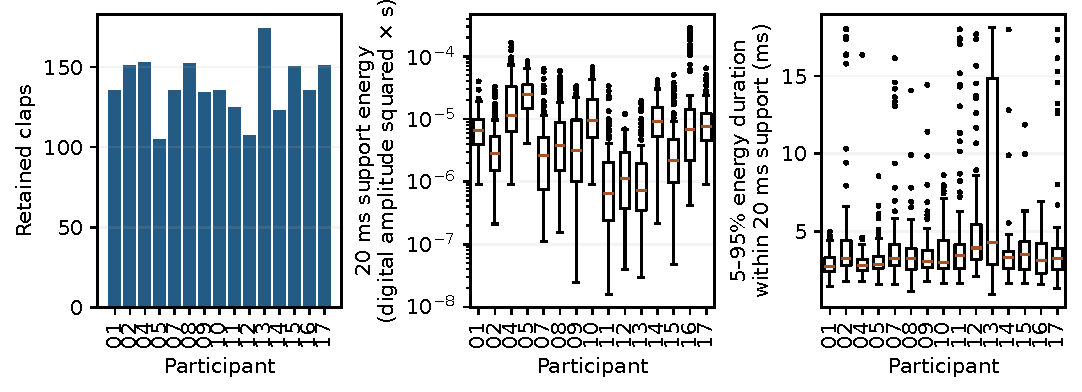
\includegraphics[width=\linewidth]{figures/e0_dataset_statistics.pdf}
%     \caption{Retained anechoic events grouped by participant: event counts,
%     digital signal energy over the 20-ms training support, and the 5--95\%
%     cumulative energy duration within that support.}
%     \label{fig:dataset-stats}
% \end{figure}

\begin{figure}[t]
   \centering
   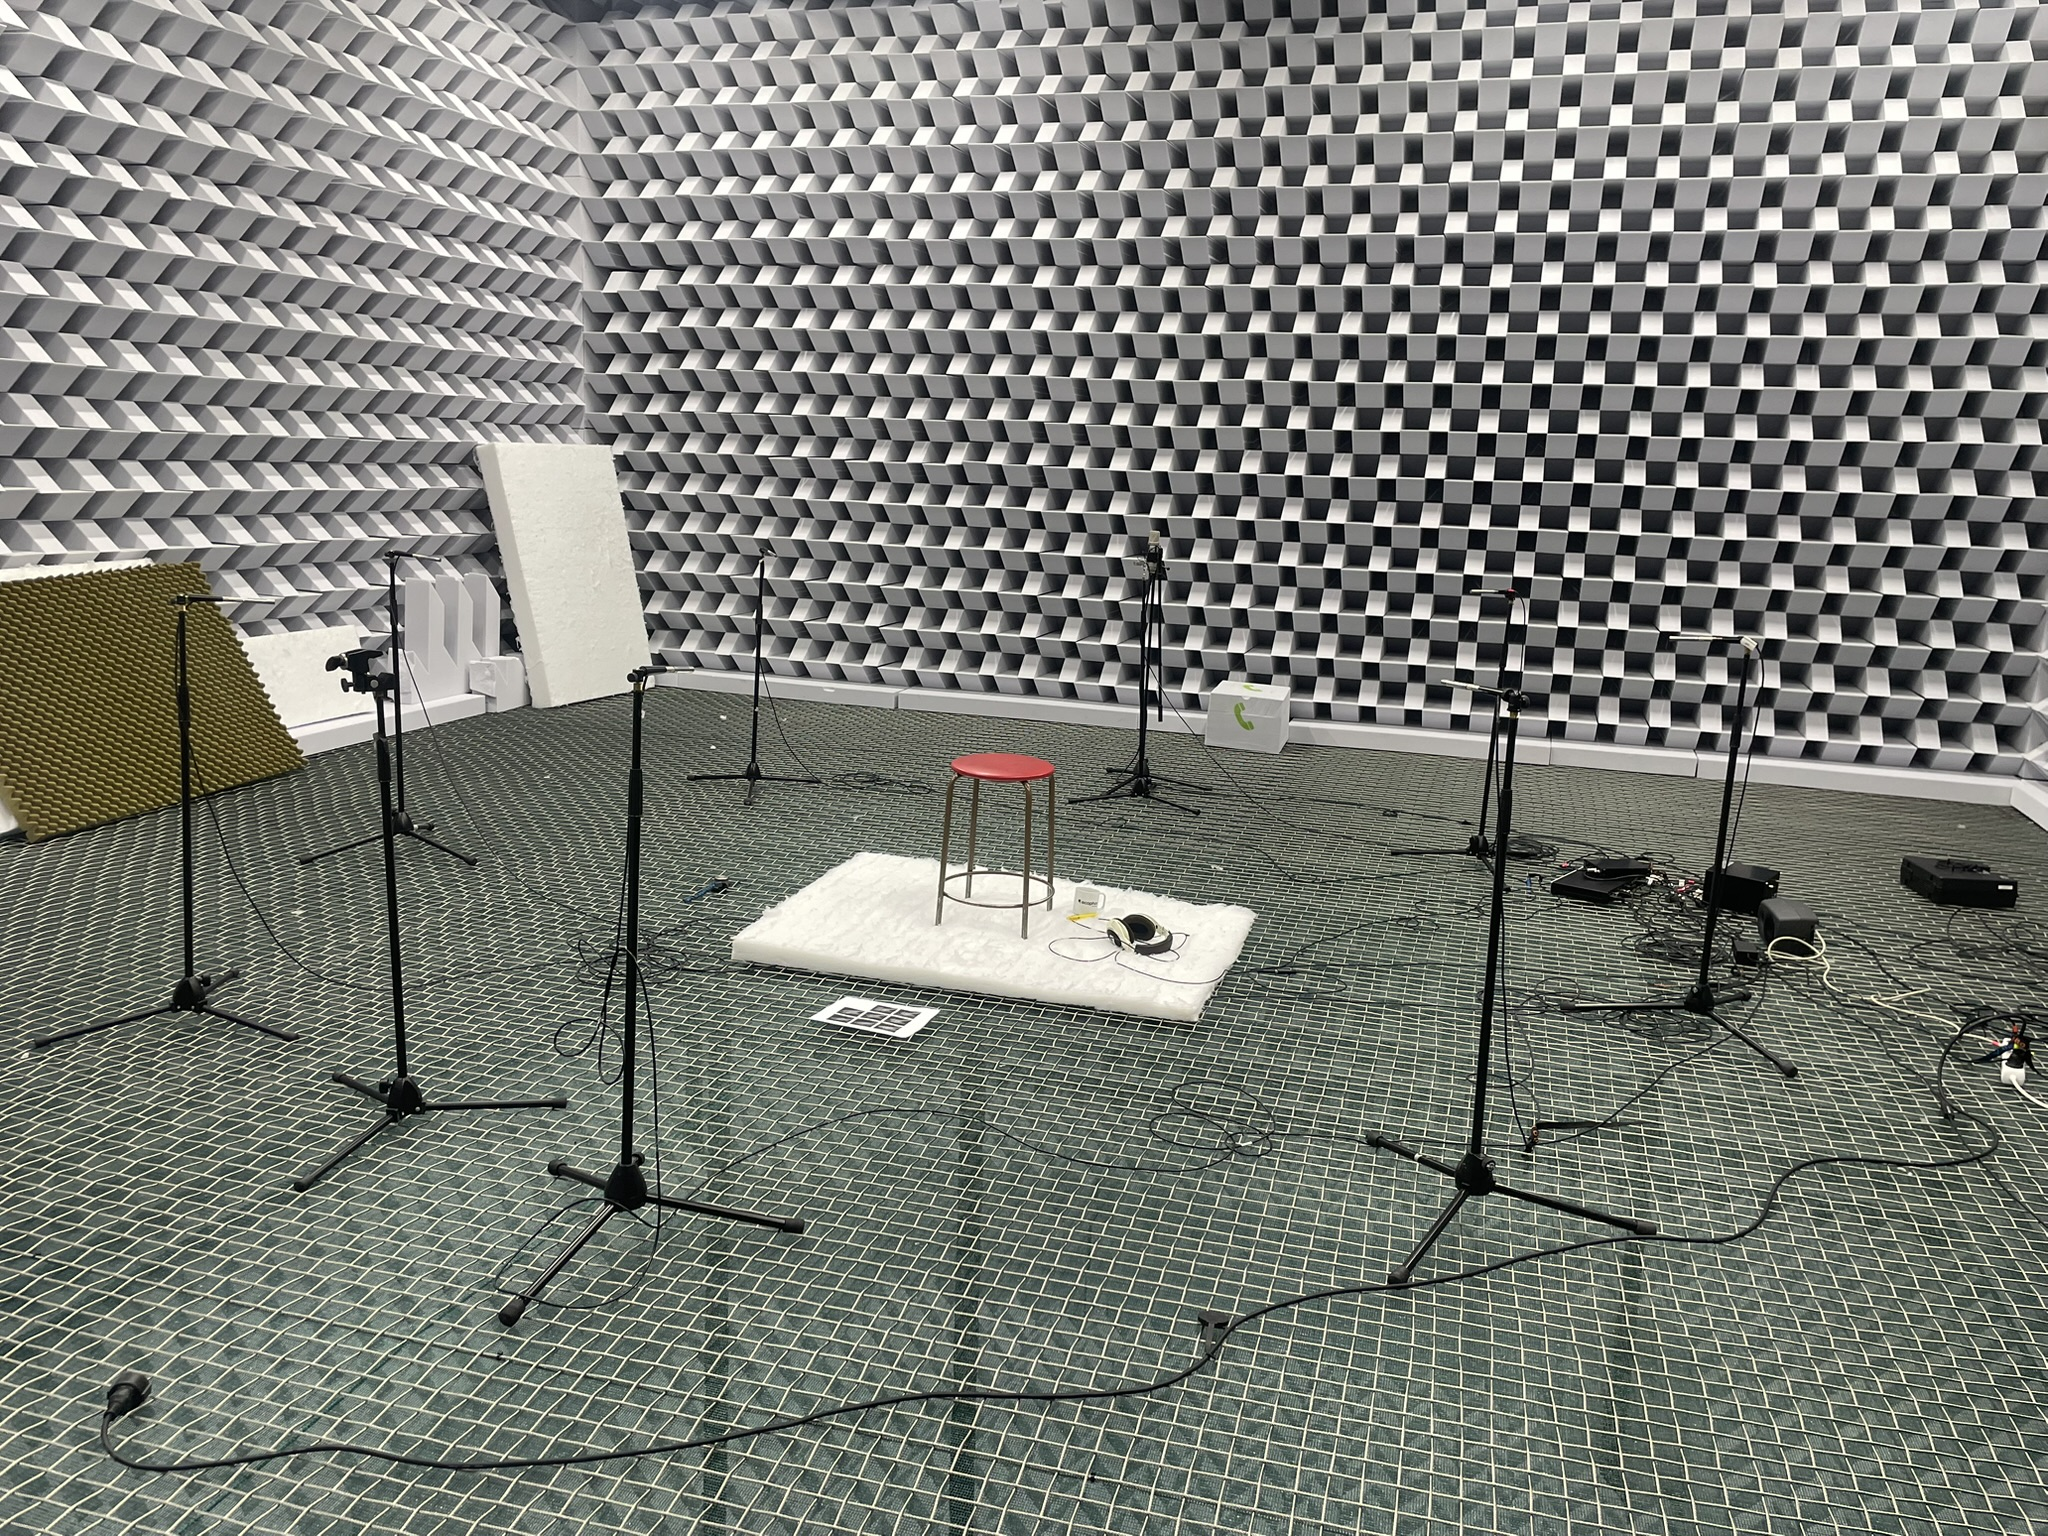
\includegraphics[width=0.7\columnwidth]{figures/clap_measurement.jpeg}
   \vspace{-0.2cm}
   \caption{Handclap recording setup in the large anechoic chamber
   at Aalto University. Participants performed natural and prescribed handclap
   configurations which were recorded using eight microphones.}
   \label{fig:clap_measurement}
   \vspace{-0.5cm}
\end{figure}

\section{Methods}
\label{sec:problem}

Let $h[t]$ denote a \ac{rir}, the signal recorded in a room when the source emits an ideal impulse, and let $y[t]$ denote the signal recorded at the same position when the excitation is a handclap instead. 
We model handclap measurements as the convolution of an unknown anechoic handclap $x[t]$ with the equally unknown \ac{rir} $h[t]$,
\begin{equation}
y[t] = (x \ast h)[t] + n[t],
\label{eq:forward}
\end{equation}
where $\ast$ denotes discrete convolution and $n[t]$ collects measurement noise and other additive perturbations. 
We write $\mathbf{y}$, $\mathbf{x}$, and $\mathbf{h}$ for the vectors collecting all samples of the corresponding signals, so that $u[t]$ is the $t$-th entry of $\mathbf{u}$. Our goal is to recover the impulse-excited \ac{rir} $\mathbf{h}\in \mathbb{R}^T$ from a single handclap measurement $\mathbf{y} \in \mathbb{R}^T$, sharing the same length $T$.
%Our goal is to recover the impulse-excited \ac{rir} $h[t]$ from the handclap room measurement $y[t]$.
%alone, with no knowledge of the handclap excitation signal.


%Controlled observations are formed by convolving an anechoic handclap with a stored RIR and adding Gaussian noise at the prescribed SNR. For measured RIR datasets, the stored responses retain the characteristics of their original measurement chain, including loudspeaker and microphone responses and measurement noise; these effects are not modeled separately.

\subsection{Identifiability and known-excitation reference}
\label{sec:notches}

We first consider the case in which the anechoic handclap excitation $x[t]$ is known. 
Let $Y[k]$, $X[k]$, $H[k]$, and $N[k]$ denote the \acp{dft} of $y[t]$, $x[t]$, $h[t]$, and $n[t]$ respectively, so that \eqref{eq:forward} becomes $Y[k]=X[k]H[k] + N[k]$.
If the measurements are noiseless, $N[k]=0$, a simple deconvolution $H[k] = Y[k]/X[k]$ recovers the RIR exactly wherever $X[k]\neq 0$.
With noise present, the same division yields
\begin{equation}
    \widehat H_{0}[k] =
    H[k]+\frac{N[k]}{X[k]},
    \label{eq:direct_noise}
\end{equation}
so the error term is inversely weighted by the excitation magnitude and grows without bound as $|X[k]|\to0$. Handclaps have deep spectral minima, as seen in Fig.~\ref{fig:dataset}, which makes this amplification severe and requires regularization.

Regularization is introduced by replacing the division with a
Tikhonov-regularized deconvolution \cite{kirkeby1999digital},
\begin{equation}
\widehat H_{\lambda}[k]
=
\frac{X^*[k]Y[k]}
{|X[k]|^{2}+\lambda},
\label{eq:tikhonov}
\end{equation}
where $(\cdot)^*$ denotes complex conjugation and $\lambda>0$ is a regularization parameter. 
At bins where $|X[k]|^{2}\gg\lambda$ the estimate reduces to direct division, whereas at the nulls, where $|X[k]|^{2}\ll\lambda$, it is driven toward zero. The parameter thus trades noise amplification against bias. The time-domain estimate follows as $\widehat h_{\lambda}[t]=\mathcal{F}^{-1}{\widehat H_{\lambda}[k]}$.
This shows that, even if $x[t]$ were known, the noise and the spectral nulls of the excitation prevent exact recovery.
%We take $\widehat h_{\lambda}[t]$ as the known-excitation reference against which blind estimation should be judged.

%This discussion shows that, even if $X[k]$ was known, the best \ac{rir} estimate we can analytically obtain $\widehat H_{\lambda}[k]$ is not exact due to the presence of noise.

With the purpose of showing how well the RIR can be recovered under ideal conditions, we evaluate both unregularized and Tikhonov-regularized deconvolution when the
anechoic handclap is known. For the unregularized control, zero-mean Gaussian noise is added at 30~dB SNR, defined using the RMS of the complete one-second clean observation. Under our digital normalization, the noise RMS averages 59.8~dB below the RIR peak for measured responses and 59.5~dB for Shoebox responses. Unregularized inversion amplifies this noise near spectral minima of the excitation. %Tikhonov regularization provides the known-excitation
%reference used in Table~\ref{tab:post-meeting-table1}, together with the 3-ms
%excitation approximation and direct regression.

\subsection{Cropped-excitation baseline}
%\subsection{Short-window excitation baseline}
\label{sec:excitation}

We now turn to the practical blind scenario in which the excitation $x[t]$ is unknown, and describe a simple baseline.
A natural approximation is to take the excitation from the measurement itself, cropping the reverberant observation to a short initial window that isolates the direct sound,
\begin{equation}
x_{\mathrm{crop}}[t]
=
y[t]\, \mathbf{1}[t<T_\mathrm{crop}],
\label{eq:crop}
\end{equation}
where $\mathbf{1}[\cdot]$ is the indicator function, equal to one when the
condition holds and zero otherwise, and $T_\mathrm{crop}$ is the window
length, set to 3 or 6~ms in our experiments.

Tikhonov-regularized deconvolution \eqref{eq:tikhonov} can then be applied with
$x_\mathrm{crop}[t]$ in place of the unknown $x[t]$. However, the approximation
$x_\mathrm{crop}[t] \approx x[t]$ is fundamentally limited. Analysis of the
recordings shows that handclaps can last more than 6~ms, so a 3-ms crop may
truncate the excitation. Extending the crop to 6~ms captures more of the
handclap, but in many rooms also includes early reflections. We therefore
evaluate both 3-ms and 6-ms crops; in either case, the direct sound cannot be
isolated by windowing alone, so $x_\mathrm{crop}[t]$ either truncates the
excitation or already contains room response.




%Table~\ref{tab:post-meeting-table1} shows that the resulting reconstruction errors are substantially larger than those obtained with the true excitation and that direct regression improves on this baseline.



\subsection{Neural regressor}

%The learned estimator receives only $y$ at inference time.
%The clean excitation $x$ is used to construct controlled training pairs and in the known-excitation reference.
%No additional noise realization is injected when constructing the controlled benchmark; recorded-handclap evaluations retain the noise present in the recordings.

We propose directly regressing the \ac{rir} from a single reverberant
handclap, $\mathbf{h}\approx \widehat{\mathbf{h}} = F_{\theta}(\mathbf{y})$, using a deep neural network $F_{\theta}$ trained in a supervised manner.
This data-driven formulation replaces the explicit forward model with a mapping learned from examples, so no estimate of the excitation is required.
Supervised training requires paired examples of measurements and their \acp{rir}, which are not available for recorded handclaps. We therefore construct pairs synthetically, drawing anechoic claps $\mathbf{x} \sim p_x$ from our dataset and \acp{rir} $\mathbf{h} \sim p_h$ from a separate corpus, and convolving them according to \eqref{eq:forward}.
The network is trained by minimizing
\begin{equation}
    \min_{\theta} \;
    \mathbb{E}_{\mathbf{x} \sim p_x, \, \mathbf{h} \sim p_h}
    \left[
        \mathcal{L} \big( \mathbf{h}, \, F_{\theta}(\mathbf{x} \ast \mathbf{h}) \big)
    \right],
    \label{eq:objective}
\end{equation}
The training loss combines waveform \ac{mse} with a magnitude-compressed STFT
loss,
\begin{equation}
\mathcal{L}(\mathbf{h},\widehat{\mathbf{h}})
=
\operatorname{MSE}\!\left(\mathbf{h},\widehat{\mathbf{h}}\right)
+
\lambda_{\mathrm{STFT}}
\operatorname{MSE}\!\left(
\Phi_{\alpha}(\mathbf{h}),
\Phi_{\alpha}(\widehat{\mathbf{h}})
\right),
\label{eq:loss}
\end{equation}
where
\[
\Phi_{\alpha}(\mathbf{z})
=
\left(
|\operatorname{STFT}(\mathbf{z})|+\epsilon
\right)^{\alpha}.
\]
For measured RIRs, both terms are evaluated only over the available
reference support, excluding zero-padding beyond the recorded target.
% We use $\lambda_{\mathrm{STFT}}=0.25$, $\alpha=2/3$, and
% $\epsilon=10^{-8}$.

% Handclaps and \acp{rir} are paired at random during training, so the network sees a different combination at each epoch. The expectation in \eqref{eq:objective} is approximated over minibatches; optimization details are given in Sec.~\ref{sec:setup}.
% For $F_{\theta}$ we adopt the two-stage hybrid architecture, originally designed for Ambisonic \ac{rir} generation 
% \cite{moliner2026ambisonics}, and reduce it to the single-channel case.
% Its two stages operate in different domains: the first estimates the full response in the time--frequency domain with a two-dimensional convolutional backbone, while a one-dimensional convolutional module refines the early response in the waveform domain.

Handclaps and \acp{rir} are paired randomly during training.
We use the two-stage time--frequency/time-domain architecture of
\cite{moliner2026ambisonics}, adapted to the single-channel case; architecture
and training details are given in Sec.~\ref{sec:model_training}.




%It is hybrid in the sense that the first stage estimates the full response in the time--frequency domain with a two-dimensional NCSN++ backbone, while a one-dimensional U-Net refines the early response in the waveform domain. The time--frequency stage uses an uncompressed complex short-time Fourier transform (STFT) representation. Differentiable inverse STFT produces a full-length coarse estimate $\widetilde h$.

%The early response is refined using a fixed boundary
%$T_{\mathrm e}=70$ ms,
%\begin{equation}
%    \widehat h_{\mathrm e}
%    =
%    U_{\phi}\!\left(
%        \mathrm{concat}\left[
%        y_{[0,T_{\mathrm e})},
%        \widetilde h_{[0,T_{\mathrm e})}
%        \right]
%      \right),
%    \label{eq:early_unet}
%\end{equation}
%where $U_{\phi}$ is a one-dimensional U-Net. The final estimate is
%\begin{equation}
%    \widehat h[t]
%    =
%    \begin{cases}
%        \widehat h_{\mathrm e}[t], & t<T_{\mathrm e},\\
%        \widetilde h[t], & t\ge T_{\mathrm e}.
%    \end{cases}
%    \label{eq:splice}
%\end{equation}


%The primary objective is waveform mean-squared error (MSE) over the available reference-RIR support. 
%For measured RIRs, a binary validity mask excludes zero-padded samples beyond the last nonzero target sample from supervision; the corresponding STFT-frame mask is applied to the auxiliary magnitude-STFT loss.
%This auxiliary loss uses $2/3$ power compression and weight $0.25$. Shoebox targets are treated as valid over the full one-second tensor during training, while the 4096-sample support restriction is applied only at evaluation. The regression model has 26.53 million active parameters.

% \subsection{Flow-Matching Comparator}

% The conditional flow-matching model uses the same two-stage architecture
% family. For target RIR $h$ and Gaussian noise $\epsilon$,
% \begin{equation}
%     h_{\tau}
%     =
%     \tau h+(1-\tau)\epsilon,
%     \qquad
%     v^{\star}
%     =
%     h-\epsilon,
%     \label{eq:flow}
% \end{equation}
% with $\tau\in[0,1]$. The model predicts
% $v_{\theta}(h_{\tau},y,\tau)$ and is trained with validity-masked waveform
% velocity MSE. The same magnitude-STFT auxiliary loss is applied to the implied
% endpoint
% \begin{equation}
%     \widetilde h_{\tau}
%     =
%     h_{\tau}+(1-\tau)
%     v_{\theta}(h_{\tau},y,\tau).
% \end{equation}

% At inference, the flow model uses a scale-aware log-SNR discretization,
% stochastic churn with $\gamma=0.5$, data-scale parameter
% $\sigma_d=0.027279$, 20 network-function evaluations (NFE), and no peak
% projection. The additional state input increases the active parameter count
% to 29.31 million.

\section{Experiments and Results}
\label{sec:setup}

% % Generated from original E3 per_example.csv + shoebox_pipeline_recheck/support_corrected.csv; aggregation unchanged.
\begin{table*}[t]
\centering\scriptsize
% \caption{Matched 1 s estimators. Provider medians aggregate draws within seed/room, then seeds within room and rooms within provider. $\dagger$ marks Shoebox: all six metrics use its retained 4096-sample (92.88 ms) support. Source reconstruction proved that longer simulated responses had been cropped before padding to 1 s; scoring was corrected on unchanged model predictions. This is not a full-second synthetic decay benchmark. Measured-provider rows are unchanged. BUT (two rooms) and ACE (one room) are descriptive. NRMSE is a companion.}
\caption{Matched 1-s regression and flow estimators. Provider medians aggregate repeated Flow draws within each seed--room pair,
then training seeds within room and rooms within provider. Shoebox
metrics use its 4096-sample (92.88-ms) valid support. BUT and ACE contain two
and one independent rooms, respectively, so those provider summaries are
descriptive. NRMSE is a companion metric.}
\label{tab:main}
\begin{tabular}{llrrrrrrrr}
\toprule
Provider & Estimator & EDC RMSE (dB) & $|\Delta C_{50}|$ (dB) & $|\Delta\mathrm{EDT}|$ (s) & EDP RMSE & Log-mag MSE & NRMSE & \# of Para. (M) & Inference \\
\midrule
Shoebox & Regression & 0.803 & 0.631 & 0.016 & 0.236 & 0.047 & 0.637 & 26.53 & 1 forward \\
Shoebox & Flow & 3.073 & 2.658 & 0.032 & 0.289 & 0.215 & 0.777 & 29.31 & 20 NFE \\
\addlinespace
MIT & Regression & 4.059 & 0.837 & 0.006 & 0.130 & 0.047 & 0.548 & 26.53 & 1 forward \\
MIT & Flow & 6.552 & 2.496 & 0.005 & 0.146 & 0.274 & 0.591 & 29.31 & 20 NFE \\
\addlinespace
BUT & Regression & 5.202 & 0.892 & 0.118 & 0.152 & 0.042 & 1.186 & 26.53 & 1 forward \\
BUT & Flow & 8.903 & 1.085 & 0.181 & 0.168 & 0.085 & 1.233 & 29.31 & 20 NFE \\
\addlinespace
ACE & Regression & 1.679 & 0.387 & 0.020 & 0.355 & 0.066 & 0.709 & 26.53 & 1 forward \\
ACE & Flow & 3.900 & 1.604 & 0.044 & 0.314 & 0.345 & 0.892 & 29.31 & 20 NFE \\
\addlinespace
OpenAIR & Regression & 2.097 & 1.262 & 0.071 & 0.104 & 0.078 & 1.199 & 26.53 & 1 forward \\
OpenAIR & Flow & 3.941 & 1.221 & 0.080 & 0.113 & 0.294 & 1.168 & 29.31 & 20 NFE \\
\addlinespace
\bottomrule
\end{tabular}
\end{table*}


% \begin{table}[t]
% \centering
% \caption{Median NRMSE by RIR source. Lower is better; $1.0$ is the error of predicting silence. Rows M1 and M2 are at $K=5$.}
% \label{tab:main}
% \begin{tabular}{llccccc}
% \toprule
%  & method & Shoebox & MIT & ACE & BUT & OpenAIR \\
% \midrule
% D1 & true clap $\to$ Tikhonov (oracle) & 0.046 & 0.025 & 0.026 & 0.078 & 0.046 \\
% D2 & \SI{3}{\milli\second} crop $\to$ Tikhonov & 4.827 & 2.684 & 2.586 & 2.022 & 2.533 \\
% S1 & hybrid regression, $K=1$ & 0.551 & 0.602 & 0.696 & 1.195 & 1.288 \\
% S2 & hybrid flow, $K=1$ (ablation) & 0.658 & 0.665 & 0.764 & 1.193 & 1.302 \\
% \midrule
% M1 & independent + average & 0.449 & 0.464 & 0.570 & 1.017 & 1.263 \\
% M2 & joint conditioning & 0.553 & 0.490 & 0.673 & 1.134 & 1.308 \\
% \bottomrule
% \end{tabular}
% \end{table}

\begin{table}[t]
\centering
\caption{Median RIR NRMSE by evaluation source. Lower is better; NRMSE $=1$ corresponds to predicting silence. M1 and M2 use $K=5$.}
\label{tab:main}
\resizebox{\columnwidth}{!}{%
\begin{tabular}{llccccc}
\toprule
 & Method & Shoebox & MIT & ACE & BUT & OpenAIR \\
\midrule
D1 & oracle Tikhonov       & 0.046 & 0.025 & 0.026 & 0.078 & 0.046 \\
D2 & \SI{3}{\milli\second} crop + Tikhonov
                             & 4.827 & 2.684 & 2.586 & 2.022 & 2.533 \\
S1 & hybrid regression     & 0.551 & 0.602 & 0.696 & 1.195 & 1.288 \\
S2 & hybrid flow           & 0.658 & 0.665 & 0.764 & 1.193 & 1.302 \\
\midrule
M1 & independent + average & 0.449 & 0.464 & 0.570 & 1.017 & 1.263 \\
M2 & joint conditioning    & 0.553 & 0.490 & 0.673 & 1.134 & 1.308 \\
\bottomrule
\end{tabular}%
}
\end{table}
% % \begin{table}[t]
% \centering\scriptsize
% \caption{Single-clap RIR estimation results. Measured RIRs pool 54
% provider/room units from 216 RIR records; Shoebox is reported separately over
% its 4096-sample (92.88-ms) valid support. Regression results are summarized
% across three training seeds. EDT uses 51 measured rooms because three MIT
% references have undefined EDT. All errors are lower-is-better; NRMSE is
% reported as a companion metric.}
% \label{tab:post-meeting-table1}
% \begin{tabular}{llrrrrrr}
% \toprule
% Population & Method & EDC (dB) & $|\Delta C_{50}|$ (dB) & $|\Delta\mathrm{EDT}|$ (s) & EDP & Log-mag MSE & NRMSE \\
% \midrule
% Measured & Known clap, unregularized & 29.05 & 10.07 & 2.524 & 0.124 & 3.416 & 0.4367 \\
% Measured & Known clap, Tikhonov & 0.8018 & 0.0236 & 0.0002436 & 0.0348 & 0.007487 & 0.01647 \\
% Measured & 3 ms crop + Tikhonov & 4.757 & 2.136 & 0.093 & 0.1665 & 0.1945 & 2.703 \\
% Measured & 1 s Regression & 3.369 & 0.9361 & 0.02042 & 0.1218 & 0.05553 & 0.5937 \\
% Shoebox & Known clap, unregularized & 2.975 & 1.656 & 0.01111 & 0.1994 & 0.0276 & 0.1359 \\
% Shoebox & Known clap, Tikhonov & 0.04272 & 0.03728 & 0.0004467 & 0.01235 & 0.002423 & 0.0457 \\
% Shoebox & 3 ms crop + Tikhonov & 2.668 & 0.7588 & 0.02552 & 0.4582 & 0.5123 & 4.881 \\
% Shoebox & 1 s Regression & 0.8026 & 0.6312 & 0.01556 & 0.2355 & 0.04675 & 0.6374 \\
% \bottomrule
% \end{tabular}
% \end{table}


%\begin{table}[t]
%\centering
%\scriptsize
%\vspace{-6.2pt}
%\caption{Single-clap RIR estimation results. Measured RIRs pool 54
%provider/room units from 216 RIR records; Simulated RIRs are reported separately over
%their 4096-sample (92.88-ms) valid support. Regression results are summarized
%across three training seeds. EDT uses 51 measured rooms because three MIT
%references have undefined EDT. All errors are lower-is-better; NRMSE is a companion metric. Known-excitation rows are oracle references; bold marks the best blind method.}
%\label{tab:post-meeting-table1}
%
%\setlength{\tabcolsep}{2.5pt}
%\renewcommand{\arraystretch}{1.05}
%
%\begin{adjustbox}{max width=\columnwidth}
%\begin{tabular}{@{}ll|cccc@{}}
%\toprule
%\textbf{Test set} & \textbf{Method}
%& \textbf{EDC}
%%& \shortstack{\boldmath$|\Delta\mathrm{EDT}|$\\\textbf{(ms)}}
%& \boldmath$|\Delta\mathrm{EDT}|$
%& \textbf{LSD}
%& \textbf{NRMSE} \\
%\midrule
%\multirow{5}{*}{Measured}
%& Known excitation, unregularized
%&$29.05\pm12.1$
%&$2524.0\pm2470.0$
%&$3.416\pm1.300$
%&$0.437\pm0.476$ \\
%
%& Known excitation
%& $0.80\pm3.67$
%& $0.2\pm6.61$
%& $0.007\pm0.0759$
%& $0.016\pm0.020$ \\
%
%& Cropped-excitation (3 ms) 
%& $4.76\pm5.09$
%& $93.0\pm98.0$
%& $0.195\pm0.265$
%& $2.703\pm0.861$ \\
%%
%& Cropped-excitation (6 ms) 
%& $7.47\pm5.64$
%& $126.0\pm121.0$
%& $9.41\pm3.64$
%& $2.960\pm0.952$ \\
%
%& Neural regressor
%& $\mathbf{3.37\pm3.51}$
%& $\mathbf{20.4\pm108.0}$
%& $\mathbf{0.056\pm0.222}$
%& $\mathbf{0.594\pm0.354}$ \\
%\midrule
%
%\multirow{5}{*}{Simulated}
%& Known excitation, unregularized
%& $2.98\pm1.27$
%& $11.1\pm11.5$
%& $0.028\pm0.0109$
%& $0.136\pm0.0488$ \\
%
%& Known excitation
%& $0.04\pm0.0403$
%& $0.4\pm0.886$
%& $0.002\pm0.00152$
%& $0.046\pm0.039$ \\
%
%& Cropped-excitation (3 ms) 
%& $2.67\pm0.762$
%& $25.5\pm67.5$
%& $0.512\pm0.0283$
%& $4.881\pm1.12$ \\
%
%& Cropped-excitation (6 ms) 
%& $1.85\pm0.405$
%& $50.9\pm64.1$
%& $14.8\pm1.82$
%& $4.240\pm0.946$ \\
%
%& Neural regressor
%& $\mathbf{0.80\pm0.305}$
%& $\mathbf{15.6\pm20.2}$
%& $\mathbf{0.047\pm0.00721}$
%& $\mathbf{0.637\pm0.249}$ \\
%\bottomrule
%\end{tabular}
%\end{adjustbox}
%\end{table}

%\begin{table}[t]
%\centering
%\scriptsize
%\caption{Single-clap RIR estimation results. Measured RIRs pool 54
%provider/room units from 216 RIR records; Shoebox is reported separately over
%its 4096-sample (92.88-ms) valid support. Regression results are summarized
%across three training seeds. EDT uses 51 measured rooms because three MIT
%references have undefined EDT. All errors are lower-is-better; NRMSE is a companion metric.
%\shih{Add Deviations!!!}}
%\label{tab:post-meeting-table1}
%
%\setlength{\tabcolsep}{2.0pt}
%\renewcommand{\arraystretch}{1.05}
%
%\begin{adjustbox}{max width=\columnwidth}
%\begin{tabular}{@{}llrrrrrr@{}}
%\toprule
%Datasets & Method 
%& \shortstack{EDC\\(dB)}
%& \shortstack{$|\Delta C_{50}|$\\(dB)}
%& \shortstack{$|\Delta\mathrm{EDT}|$\\(s)}
%& EDP
%& \shortstack{Log-mag\\MSE}
%& NRMSE \\
%\midrule
%%Measured & Known clap, unregularized
%& 29.05 & 10.07 & 2.524 & 0.124 & 3.416 & 0.4367 \\
%Measured & Known clap, Tikhonov
%& 0.8018 & 0.0236 & 0.0002436 & 0.0348 & 0.007487 & 0.01647 \\
%Measured & 3 ms crop + Tikhonov
%& 4.757 & 2.136 & 0.093 & 0.1665 & 0.1945 & 2.703 \\
%Measured & 1 s Regression
%& 3.369 & 0.9361 & 0.02042 & 0.1218 & 0.05553 & 0.5937 \\
%\midrule
%Shoebox & Known clap, unregularized
%& 2.975 & 1.656 & 0.01111 & 0.1994 & 0.0276 & 0.1359 \\
%Shoebox & Known clap, Tikhonov
%& 0.04272 & 0.03728 & 0.0004467 & 0.01235 & 0.002423 & 0.0457 \\
%Shoebox & 3 ms crop + Tikhonov
%& 2.668 & 0.7588 & 0.02552 & 0.4582 & 0.5123 & 4.881 \\
%Shoebox & 1 s Regression
%& 0.8026 & 0.6312 & 0.01556 & 0.2355 & 0.04675 & 0.6374 \\
%\bottomrule
%\end{tabular}
%\end{adjustbox}
%\end{table}
%


\subsection{Training data and controlled benchmark}
\label{sec:data}

% Reverberant handclaps for training and testing are synthesized by convolving anechoic handclaps from the dataset in Sec.~\ref{sec:dataset} with both simulated and measured \acp{rir}.
% The simulated \acp{rir} and the MIT, BUT, and ACE corpora are used for training, with room-disjoint train/validation/test splits; OpenAIR is held out entirely as an unseen \ac{rir} source.
% Measured \acp{rir} are taken from four public corpora: MIT~\cite{mit}, BUT~\cite{but}, ACE~\cite{ace}, and OpenAIR~\cite{OpenAIR}.
% The simulated \acp{rir} and the MIT, BUT, and ACE corpora are used for training, with room-disjoint train/validation/test splits; OpenAIR is used for testing only.
% At most 16 \acp{rir} are used per room and split, giving 372 training \acp{rir} (24 simulated, 172 MIT, 96 BUT from six rooms, and 80 ACE from five rooms).
Reverberant handclaps are synthesized by convolving anechoic claps with
simulated Shoebox RIRs and measured RIRs from MIT, BUT, ACE, and OpenAIR
\cite{mit,but,ace,OpenAIR}. Shoebox, MIT, BUT, and ACE are used for training
with room-disjoint splits, while OpenAIR is reserved for testing.
At most 16 RIRs are used per room and split.
All \acp{rir} are resampled to 44.1~kHz, trimmed to start at their onset, truncated or zero-padded to 1~s, and peak-normalized.
Each \ac{rir} is convolved with five handclaps drawn from the participants of the corresponding split, and each observation is peak-normalized.
The handclap split is participant-disjoint: 453 claps from three held-out participants (P08, P15, and P17) form the test pool.
The resulting test set contains 220 clap--\ac{rir} observations (216 measured and four simulated \acp{rir}), using 184 distinct claps from the held-out pool.

\subsection{Model architecture and training details} \label{sec:model_training}

For $F_\theta$, we reimplement the hybrid architecture of \cite{moliner2026ambisonics}, originally proposed for Ambisonics encoding of multichannel \acp{rir}, and adapt it to a single-channel input and output: the network takes a one-second reverberant handclap and outputs the corresponding one-second \ac{rir}.
The first stage computes an STFT with a 510-sample Hann window and a hop of 128 samples.
 A 2D convolutional NCSN++ network \cite{song2021sde} (25.0M parameters) processes the real and imaginary parts of this complex STFT, and an inverse STFT of its output gives a coarse estimate of the full response.
The second stage consists of a 1D U-Net (1.5M parameters) operating on the waveform, which refines the split early reflections (using a mixing time of $\sim$70~ms).
Its output is added to the output of the first stage. 


The loss in \eqref{eq:loss} uses $\lambda_{\mathrm{STFT}}=0.25$, $\alpha=2/3$, and $\epsilon=10^{-8}$, with the STFT computed using a 510-sample Hann window and a 127-sample hop.
 Both loss terms are restricted to the valid support of the recording, so the zero-padding applied to measured \acp{rir} which files had been cropped shorter than 1\,s does not contribute to the gradient. 
Optimization uses AdamW \cite{loshchilov2019adamw} with a constant learning rate of $2\times10^{-4}$, gradient-norm clipping at 1, an effective batch size of 16, and 20,000 updates. 
%No additional observation-noise augmentation is applied during training.
Full training details are available in the accompanying code.
%For the model architecture $F_\theta$, we reimplement the the design specified in \cite{moliner2026ambisonics}.
%The time--frequency stage uses an uncompressed complex STFT with a 510-sample Hann window and 128-sample hop, followed by a 2D-convolutional U-Net-style module, particularly NCSN++ \cite{song2021sde} with 24.98 million paramters.
%with 128 base channels, channel multipliers $(1,2,2,2)$, and one residual block per resolution.
%An inverse STFT produces the coarse full-response estimate, and a five-level 1D U-Net (1.55 million parameters) refines its first 3072 samples (69.66~ms), corresponding to the early reflections. The refined early reflections are then summed to the output of the first stage.
%Optimization uses AdamW with a constant learning rate of $2\times10^{-4}$ and gradient-norm clipping at 1.
%Training runs for 20,000 optimizer updates with an effective batch size of 16, implemented using micro-batches of two examples and eight gradient-accumulation steps per update. 
%No additional observation-noise augmentation is applied during training.
%\subsection{Controlled handclap deconvolution benchmark}
%We design a controlled benchmark built by convolving \acp{rir} with anechoic handclap recordings.
%The controlled benchmark uses five RIR sources: procedurally generated Shoebox responses and measured MIT ~\cite{mit}, BUT ~\cite{but}, ACE ~\cite{ace}, and OpenAIR ~\cite{OpenAIR} responses.
%The anechoic handclap split is participant-disjoint. The anechoic handclap split is participant-disjoint. A total of 453 claps from three held-out participants (P08, P15, and P17) form the test pool.
%The controlled benchmark contains 220 clap--RIR observations, comprising 216 measured and four simulated RIR records; these observations use 184 distinct claps drawn from the held-out pool.
%Shoebox, MIT, BUT, and ACE are used for training; OpenAIR is held out as an unseen RIR provider.
%The remaining providers use dataset-specific room-disjoint or configuration-disjoint splits.
%The regression estimator predicts a one-second RIR and uses peak-normalized targets, an effective batch size of 16, and 20,000 optimization updates.
%Measured RIRs use per-example validity masks so that unavailable recording tails do not contribute to the loss.
%Multi-resolution STFT supervision is disabled.
%The magnitude-STFT loss uses $\alpha=2/3$ power compression, $\lambda_{\mathrm{STFT}}=0.25K$, where $K$ is the number of STFT frequency bins, and $\epsilon=10^{-8}$.
%Shoebox targets are treated as valid over the full one-second tensor during training, while the 4096-sample support restriction is applied only at evaluation.
%The regression model has 26.53 million active parameters.
% Evaluation is restricted to valid reference support. 
% The stored Shoebox targets contain 4096 valid samples, corresponding to 92.88 ms, followed by padding, so Shoebox metrics use only those 4096 samples.
% For the measured RIR sources, records are first summarized within room and training seed, then across the three Regression seeds and across provider/room units.
% The pooled measured benchmark contains 54 such units; EDT uses 51 because three MIT reference RIRs have undefined EDT.
Measured-RIR results are summarized within room and training seed, then across
the three Regression seeds and provider/room units. The pooled benchmark
contains 54 units; EDT uses 51 because three MIT references have undefined EDT.



%\begin{figure}[t]
%    \centering
%    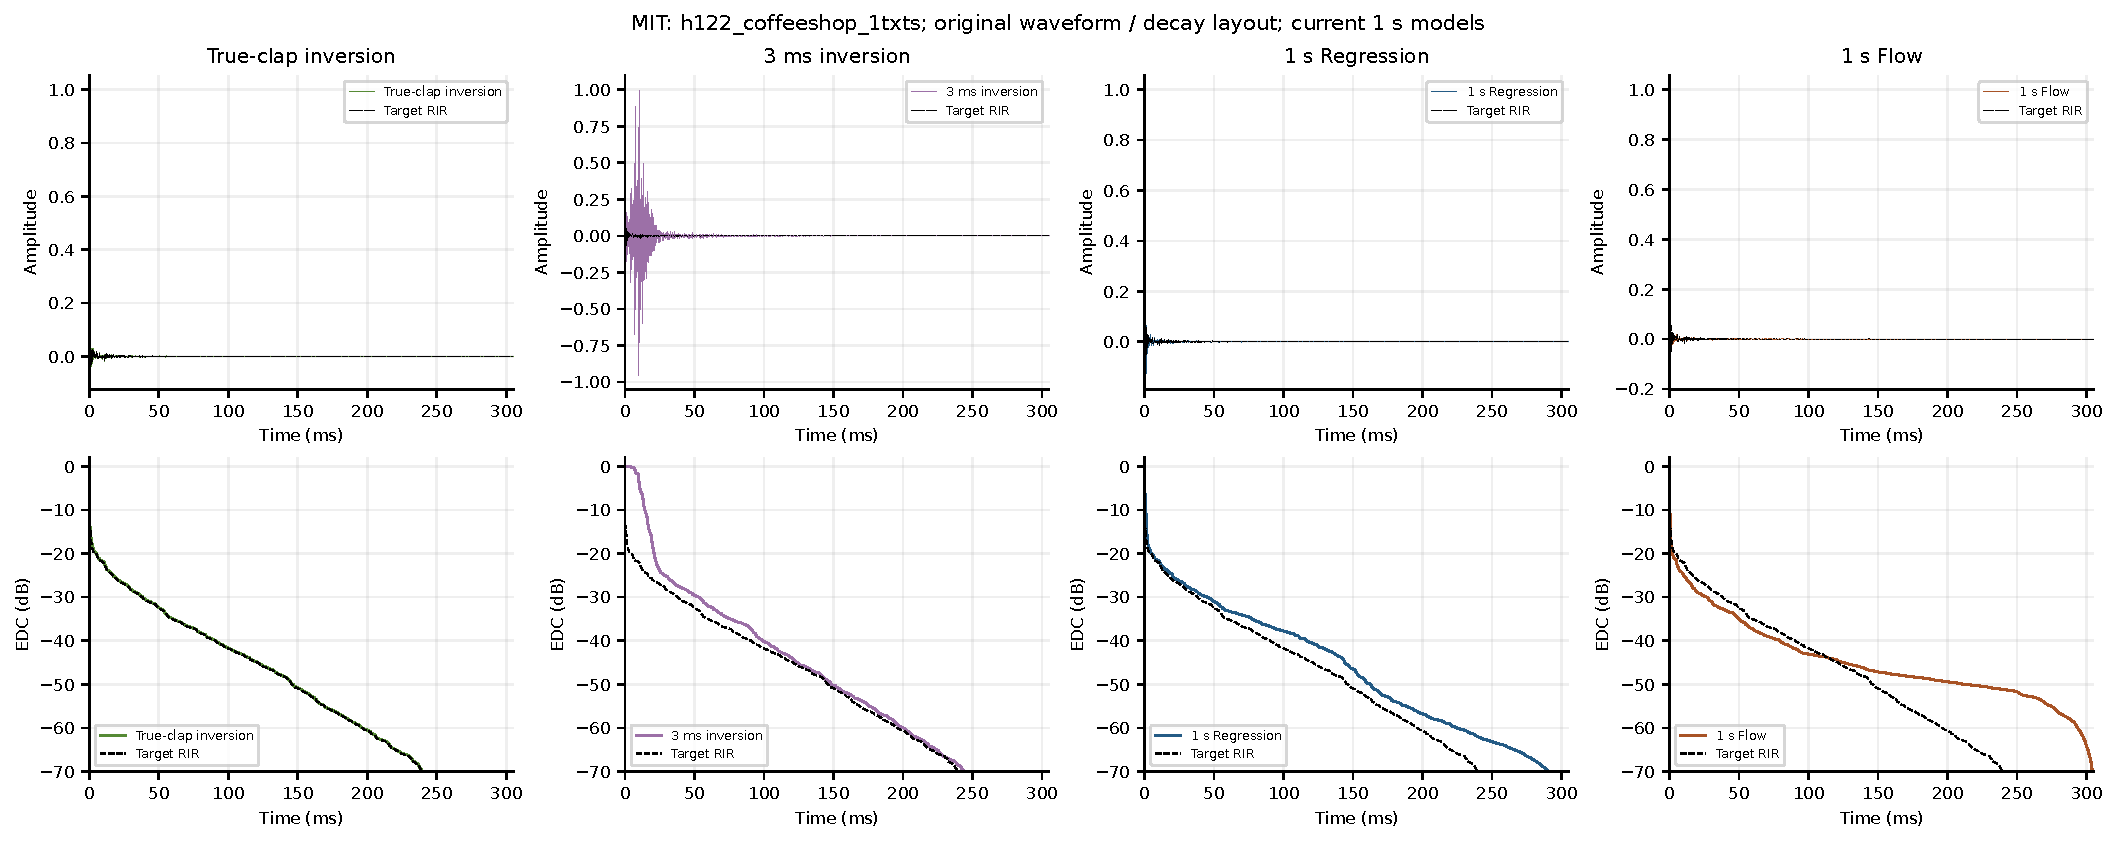
\includegraphics[width=\linewidth]{figures/paper_fig1_oracle_crop_hybrid.pdf}
%    \caption{Representative held-out MIT example comparing known-excitation
%    inversion, the 3-ms excitation approximation, direct Regression, and
%    conditional Flow matching. The top row shows waveform estimates and the
%    bottom row their energy-decay curves. Known-excitation inversion closely
%    follows the reference RIR, whereas the 3-ms approximation introduces large
%    reconstruction error. Regression better preserves the reference decay than
%    the matched Flow estimator in this example.}
%    \label{fig:single_example}
%\end{figure}

% \subsection{Matched Regression--Flow Comparison}

% Regression and flow matching use the same horizon, uncompressed complex-STFT
% representation, training data, target normalization, validity handling,
% effective batch size, training budget, seeds, and magnitude-STFT auxiliary
% loss. Their primary objectives differ by construction: regression predicts the
% RIR with waveform MSE, whereas flow matching predicts the velocity field with
% velocity MSE. Regression requires one deterministic forward pass. Flow uses
% the sampler described above with 20 NFE. Both models are evaluated with the
% same reference support and metric definitions.

% \subsection{Recorded-Clap Evaluation}


% The Spheres dataset \cite{sphere} provides handclap recordings and
% sweep-derived reference RIRs at matched source-position/microphone locations.
% We evaluate 51 such pairs. The common observation/reference support is 250 ms,
% so the one-second model input is padded where necessary while all
% reference-based metrics are restricted to the available 250-ms support.

% The phone evaluation contains 280 protocol claps recorded with an iPhone 15 across seven rooms,
% eight clap modes, and five repetitions per mode. These recordings have no
% paired reference RIR. They are therefore used to quantify within-room
% prediction consistency rather than reconstruction accuracy.


\subsection{Evaluation metrics}
\label{sec:metrics}

We report four reference-based metrics comparing the estimated \ac{rir}
$\widehat{\mathbf{h}}$ with the corresponding reference $\mathbf{h}$:
normalized broadband energy-decay-curve (EDC) error in decibels, absolute
early-decay-time (EDT) error, log-spectral mean-squared error, and waveform
normalized root-mean-square error (NRMSE).

For the normalized broadband EDC metric, the last 0.5\% of each signal is
discarded before computing the broadband Schroeder energy decay
\begin{equation}
E_h[n]
=
\sum_{u=n}^{L_h-1} h^2[u],
\end{equation}
where $L_h$ is the retained signal length. The decay is converted to decibels
as
\begin{equation}
D_h[n]
=
10\log_{10}\!\left(E_h[n]+\epsilon\right),
\qquad \epsilon=10^{-32}.
\end{equation}
Each decay curve is referred to its own initial level,
\begin{equation}
\widetilde D_h[n]
=
D_h[n]-D_h[0].
\end{equation}
The normalized broadband EDC error is reported in decibels as
\begin{equation}
\mathcal{L}_{\mathrm{EDC}}^{\mathrm{dB}}
=
10\log_{10}\!\left(
\frac{
\operatorname{MSE}\!\left(
\widetilde D_{\widehat h},
\widetilde D_h
\right)}
{
\operatorname{mean}\!\left(
\widetilde D_h^{\,2}
\right)}
\right).
\label{eq:edc}
\end{equation}
Because each decay curve is referred to its own initial level,
$\mathcal{L}_{\mathrm{EDC}}^{\mathrm{dB}}$ is invariant to overall gain and
measures normalized broadband decay-shape error. More negative values
indicate lower error.

EDT is estimated from the initial Schroeder decay and reported as
$|\mathrm{EDT}(\widehat h)-\mathrm{EDT}(h)|$ in milliseconds.
Log-spectral error is the mean-squared difference between the predicted and
reference log-magnitude STFTs. Waveform error is
\begin{equation}
\mathrm{NRMSE}(\widehat h,h)
=
\frac{\|\widehat h-h\|_2}{\|h\|_2},
\label{eq:nrmse}
\end{equation}
where lower values indicate smaller waveform error.



\subsection{Controlled single-handclap results}
\begin{table}[t]
\vspace{-6.2pt}
\caption{Single-clap RIR estimation results (mean $\pm$ std.).
For normalized broadband EDC, more negative values indicate lower error.
Known-excitation rows are references; best unknown-excitation result per
metric and block is shown in bold.}
\label{tab:post-meeting-table1}

\resizebox{\columnwidth}{!}{%
\centering
\begin{tabular}{@{}ll|cccc@{}}
\toprule
& \textbf{Method}
& \textbf{EDC (dB)} $\downarrow$
& {\boldmath$|\Delta\mathrm{EDT}|$} $\downarrow$
& \textbf{Log-Spec MSE} $\downarrow$
& \textbf{NRMSE} $\downarrow$ \\
\midrule \midrule

\multirow{5}{*}{\textit{Measured}}
& Known exc. (unreg.)
& $-3.2${\scriptsize$\,\pm\,1.7$}
& 2500{\scriptsize$\,\pm\,2500$}
& 3.4{\scriptsize$\,\pm\,1.3$}
& 0.44{\scriptsize$\,\pm\,0.48$} \\

& Known exc.
& $-39.5${\scriptsize$\,\pm\,16.7$}
& 0.2{\scriptsize$\,\pm\,6.6$}
& 0.007{\scriptsize$\,\pm\,0.076$}
& 0.016{\scriptsize$\,\pm\,0.020$} \\
\cmidrule{2-6}

& Cropped exc. (3 ms)
& $-18.3${\scriptsize$\,\pm\,6.3$}
& 93{\scriptsize$\,\pm\,98$}
& 0.20{\scriptsize$\,\pm\,0.27$}
& 2.7{\scriptsize$\,\pm\,0.86$} \\

& Cropped exc. (6 ms)
& $-17.4${\scriptsize$\,\pm\,6.0$}
& 130{\scriptsize$\,\pm\,120$}
& 9.4{\scriptsize$\,\pm\,3.6$}
& 3.0{\scriptsize$\,\pm\,0.95$} \\

& Neural regressor
& \textbf{$-$21.7}{\scriptsize$\,\pm\,5.7$}
& \textbf{20}{\scriptsize$\,\pm\,110$}
& \textbf{0.056}{\scriptsize$\,\pm\,0.22$}
& \textbf{0.59}{\scriptsize$\,\pm\,0.35$} \\
\midrule \midrule

\multirow{5}{*}{\textit{Simulated}}
& Known exc. (unreg.)
& $-17.2${\scriptsize$\,\pm\,4.7$}
& 11{\scriptsize$\,\pm\,12$}
& 0.028{\scriptsize$\,\pm\,0.011$}
& 0.14{\scriptsize$\,\pm\,0.049$} \\

& Known exc.
& $-49.7${\scriptsize$\,\pm\,6.3$}
& 0.4{\scriptsize$\,\pm\,0.89$}
& 0.002{\scriptsize$\,\pm\,0.0015$}
& 0.046{\scriptsize$\,\pm\,0.039$} \\
\cmidrule{2-6}

& Cropped exc. (3 ms)
& $-17.7${\scriptsize$\,\pm\,1.0$}
& 26{\scriptsize$\,\pm\,68$}
& 0.51{\scriptsize$\,\pm\,0.028$}
& 4.9{\scriptsize$\,\pm\,1.1$} \\

& Cropped exc. (6 ms)
& $-19.8${\scriptsize$\,\pm\,1.1$}
& 51{\scriptsize$\,\pm\,64$}
& 15{\scriptsize$\,\pm\,1.8$}
& 4.2{\scriptsize$\,\pm\,0.95$} \\

& Neural regressor
& \textbf{$-$27.9}{\scriptsize$\,\pm\,2.2$}
& \textbf{16}{\scriptsize$\,\pm\,20$}
& \textbf{0.047}{\scriptsize$\,\pm\,0.0072$}
& \textbf{0.64}{\scriptsize$\,\pm\,0.25$} \\
\bottomrule
\end{tabular}%
}
\vspace{-0.3cm}
\end{table}




On the pooled measured RIRs, known-handclap unregularized inversion gives a
normalized broadband EDC error of $-3.2$~dB under 30-dB-SNR additive noise,
whereas Tikhonov-regularized inversion gives $-39.5$~dB in the noiseless
condition. With unknown excitation, the 3-ms and 6-ms cropped-excitation
baselines give $-18.3$ and $-17.4$~dB, respectively. These results illustrate
the limitation of direct-sound windowing: short crops truncate the handclap,
while longer crops may include early reflections.

Direct regression improves the measured-RIR EDC error to $-21.7$~dB and also
gives lower EDT, log-spectral MSE, and NRMSE errors than both
cropped-excitation baselines, although a gap to known-excitation deconvolution
remains. On the simulated set, the 6-ms crop improves the normalized
broadband EDC error from $-17.7$ to $-19.8$~dB relative to the 3-ms crop,
while direct regression gives the lowest unknown-excitation error at
$-27.9$~dB and lower error across all reported metrics. The measured RIR
targets retain the loudspeaker and measurement-chain responses of their source
datasets, so the regressor may also absorb dataset-specific system coloration.

%\begin{figure}[t]
%    \centering
%    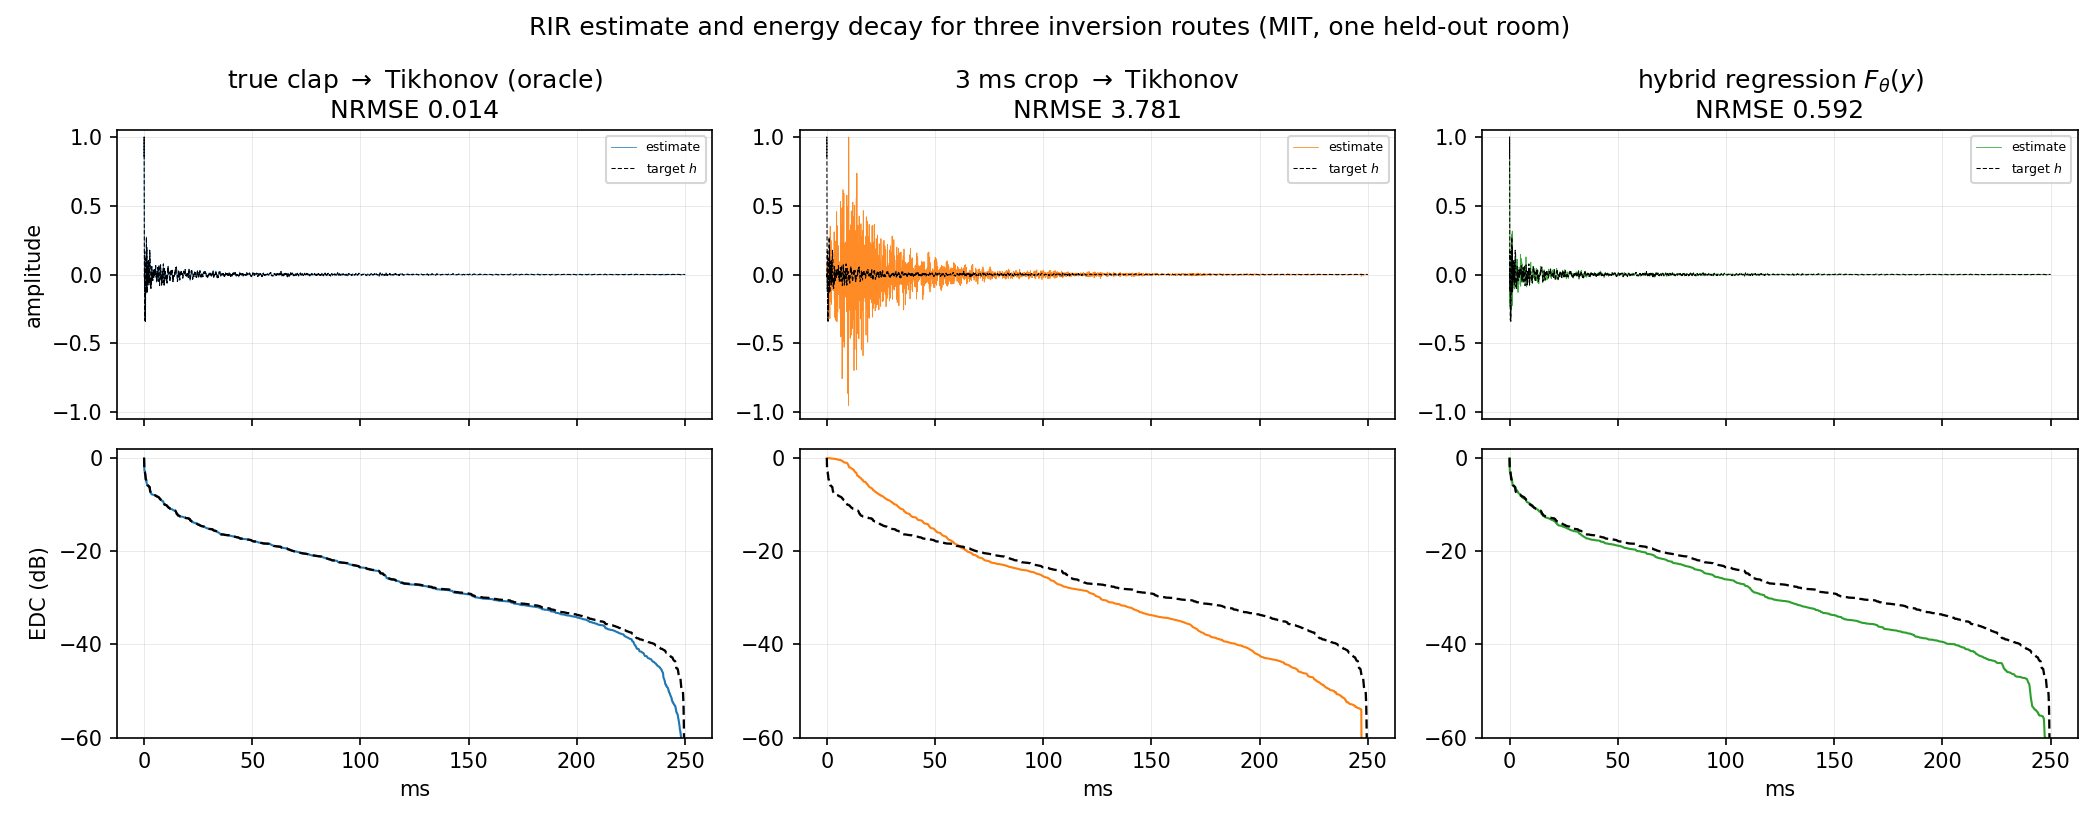
\includegraphics[width=0.5\textwidth]{figures/fig1_oracle_crop_hybrid.png}
%    \caption{One held-out MIT example. Known-clap Tikhonov inversion closely
%    reproduces the target, the 3-ms crop produces large waveform and decay
%    errors, and direct regression recovers the main response structure.}
%    \label{fig:single_example}
%\end{figure}

\subsection{Real-world transfer: qualitative phone-recording example}
\label{sec:real}

% \kyung{Only add 1 qualitative example. Explain briefly how the recording was done. [Done]}

% \subsection{Spheres: Paired Sweep-Reference Evaluation}

% At each of 51 Spheres source-position/microphone pairs, we estimate the RIR
% from one recorded handclap and compare it with the paired sweep-derived
% reference. The observation and reference provide 250 ms of common support.
% Inputs are padded to the one-second model horizon, while scoring is restricted
% to the observed 250 ms.

% Averaging the three training-seed means gives EDC RMSE \EfiveEDC{} dB,
% absolute $C_{50}$ error \EfiveC{} dB, and absolute EDT error
% \EfiveEDT{} s. These errors indicate a substantial remaining real-recording
% transfer gap. Figure~\ref{fig:spheres-examples} shows three pairs selected by
% the Regression EDC-error distribution. For qualitative comparison, the figure
% also includes one flow-matching sample from training seed 42001; quantitative
% Spheres results use the selected regression estimator.

% \begin{figure}[t]
%     \centering
%     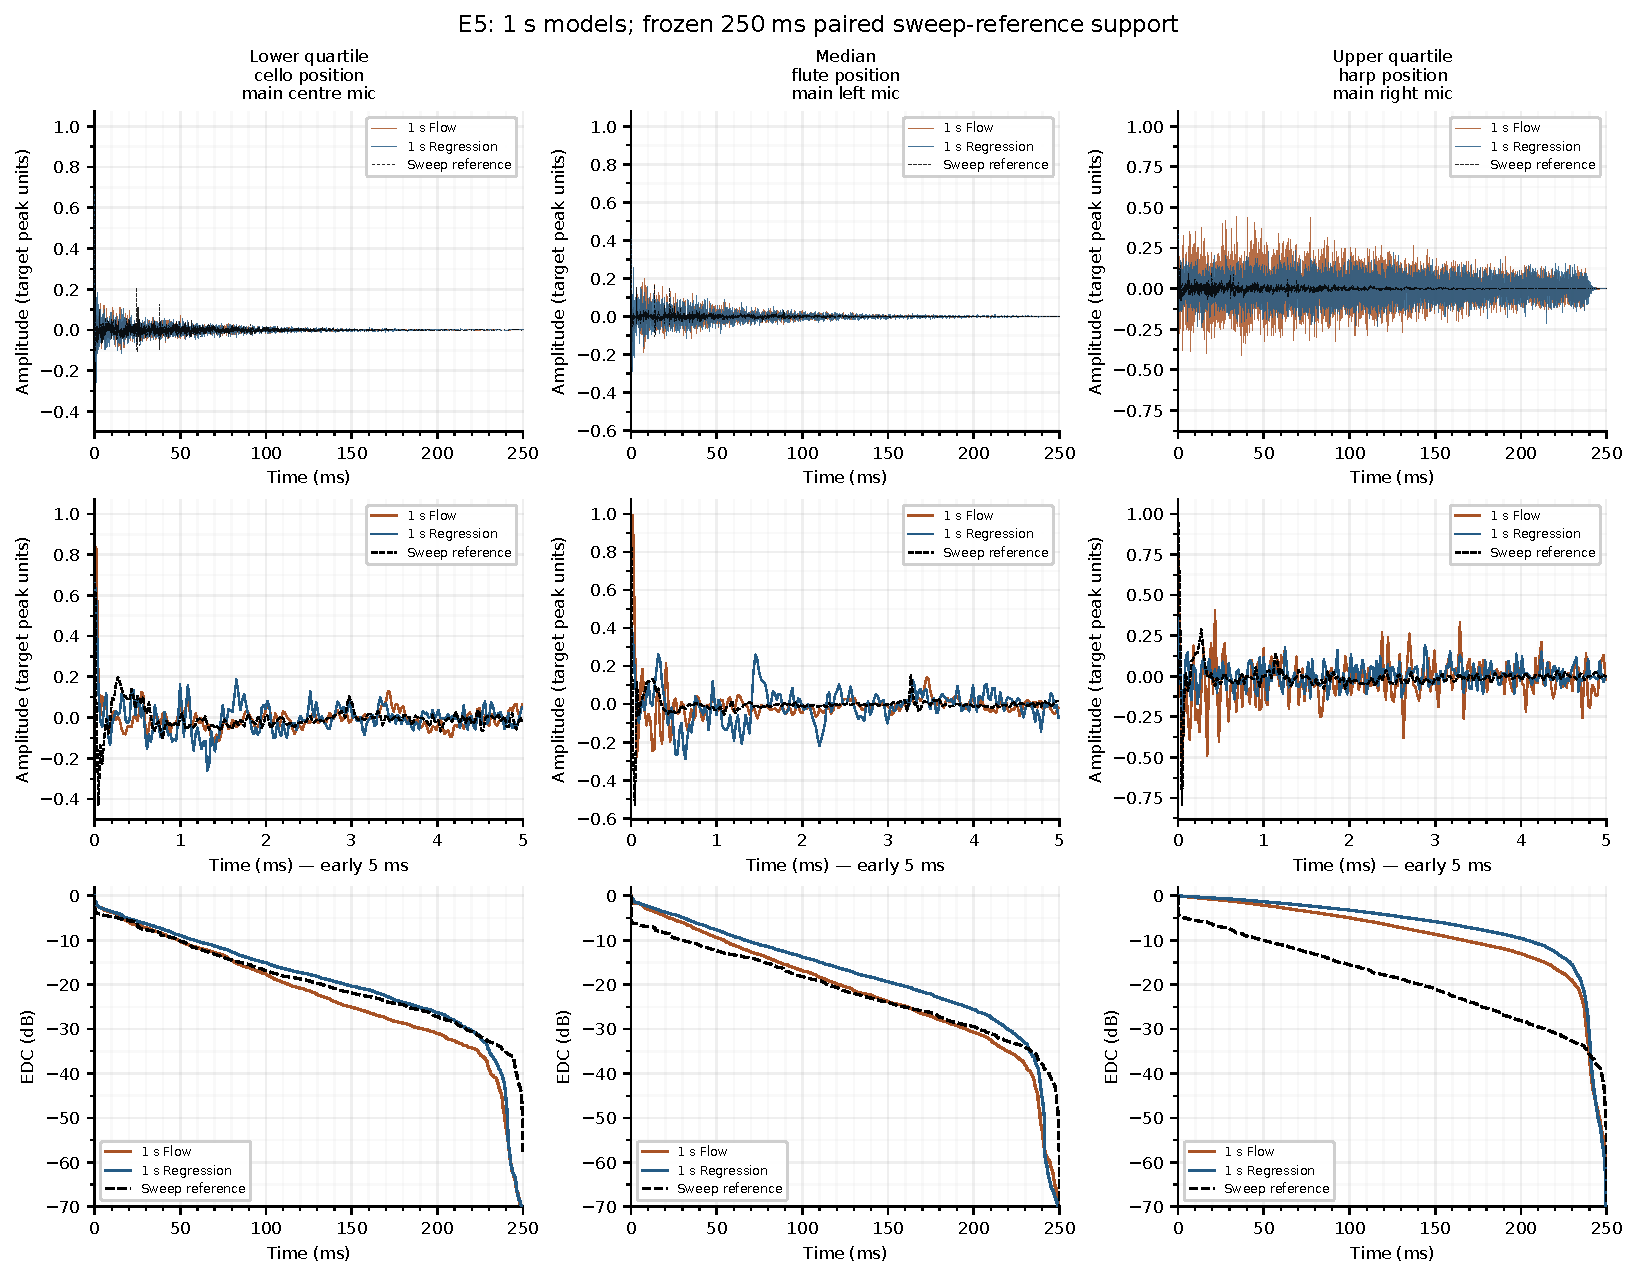
\includegraphics[width=\linewidth]{figures/e5_examples.pdf}
%     \caption{Spheres examples at the lower quartile, median, and upper quartile
%     of Regression EDC RMSE across training seeds. Each column shows the
%     250-ms waveform, first 5 ms, and EDC. Regression and one flow-matching
%     sample from seed 42001 are compared with the paired sweep-derived reference.}
%     \label{fig:spheres-examples}
% \end{figure}

% % \begin{figure}[t]
% %     \centering
% %     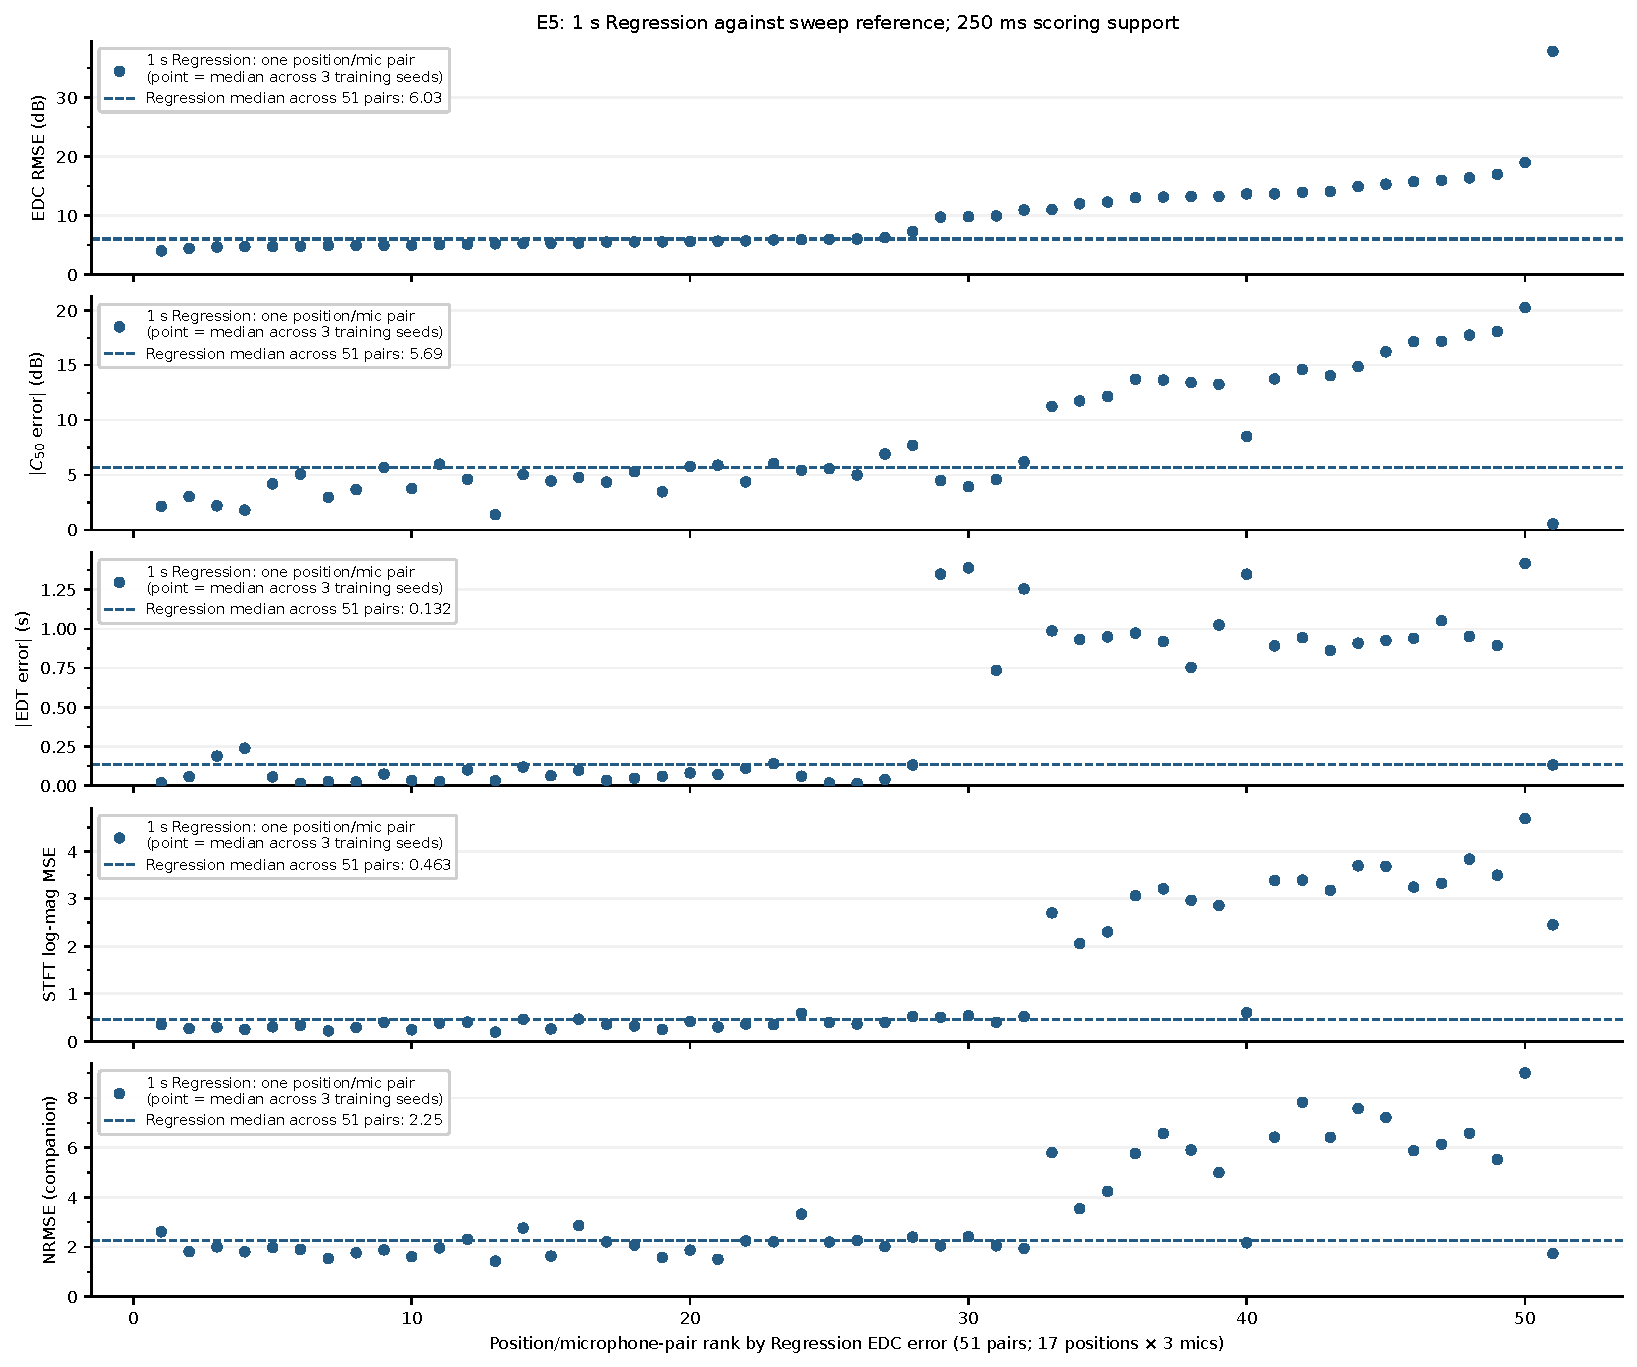
\includegraphics[width=\linewidth]{figures/e5_real_clap_transfer.pdf}
% %     \caption{Paired Spheres transfer for the selected one-second Regression
% %     model. Each point is one source-position/microphone pair and is the median
% %     across three training seeds. Pairs are ranked by EDC RMSE. Dashed lines
% %     show the median across all 51 pairs. All metrics use the common 250-ms
% %     reference support; NRMSE is a companion metric.}
% %     \label{fig:spheres-distribution}
% % \end{figure}

% \subsection{ARPEGE: external paired real-room evaluation}

% We further evaluate external transfer on the ARPEGE dataset, which provides
% recorded handclaps and measured RIRs with annotated source and receiver
% geometry. ARPEGE is used only for evaluation and is not included in training
% or fine-tuning.

% The evaluation contains 56 recorded-clap/receiver pairs from 28 source-position
% configurations across six rooms. For each long recording, the first eligible
% isolated clap is selected before inference using the same isolation criterion
% as the Spheres evaluation. The observation and measured reference RIR are
% resampled to 44.1 kHz and aligned independently from their recorded onsets.
% The first physical microphone capsule is used without channel averaging.
% No denoising, reference-guided alignment, output gain fitting, or delay fitting
% is applied.

% We evaluate the final one-second Regression and Flow models using seed 42001.
% Flow uses one sample with the same 20-NFE inference procedure used in the
% matched model comparison. Because this evaluation uses a single training seed,
% the results are descriptive and do not estimate training-seed uncertainty.

% Across room-level medians, Regression obtains an EDC RMSE of 4.487 dB,
% an absolute $C_{50}$ error of 1.61 dB, an absolute EDT error of 0.07789 s,
% an EDP RMSE of 0.4679, a log-magnitude STFT MSE of 0.4154, and an NRMSE
% of 1.338. The corresponding Flow values are 10.3 dB, 1.18 dB, 0.1549 s,
% 0.4477, 0.4503, and 1.373, respectively. Regression therefore gives
% substantially lower decay error and lower EDT and spectral errors, while Flow
% has lower $C_{50}$ and EDP errors on this external set.

% These results confirm that external paired-clap transfer remains imperfect.
% The measured reference is produced by a loudspeaker at the annotated source
% position, whereas the handclap has unknown and different directivity.
% Consequently, geometric pairing does not imply waveform identity between the
% handclap excitation and the reference measurement.

% \begin{figure}[t]
%     \centering
%     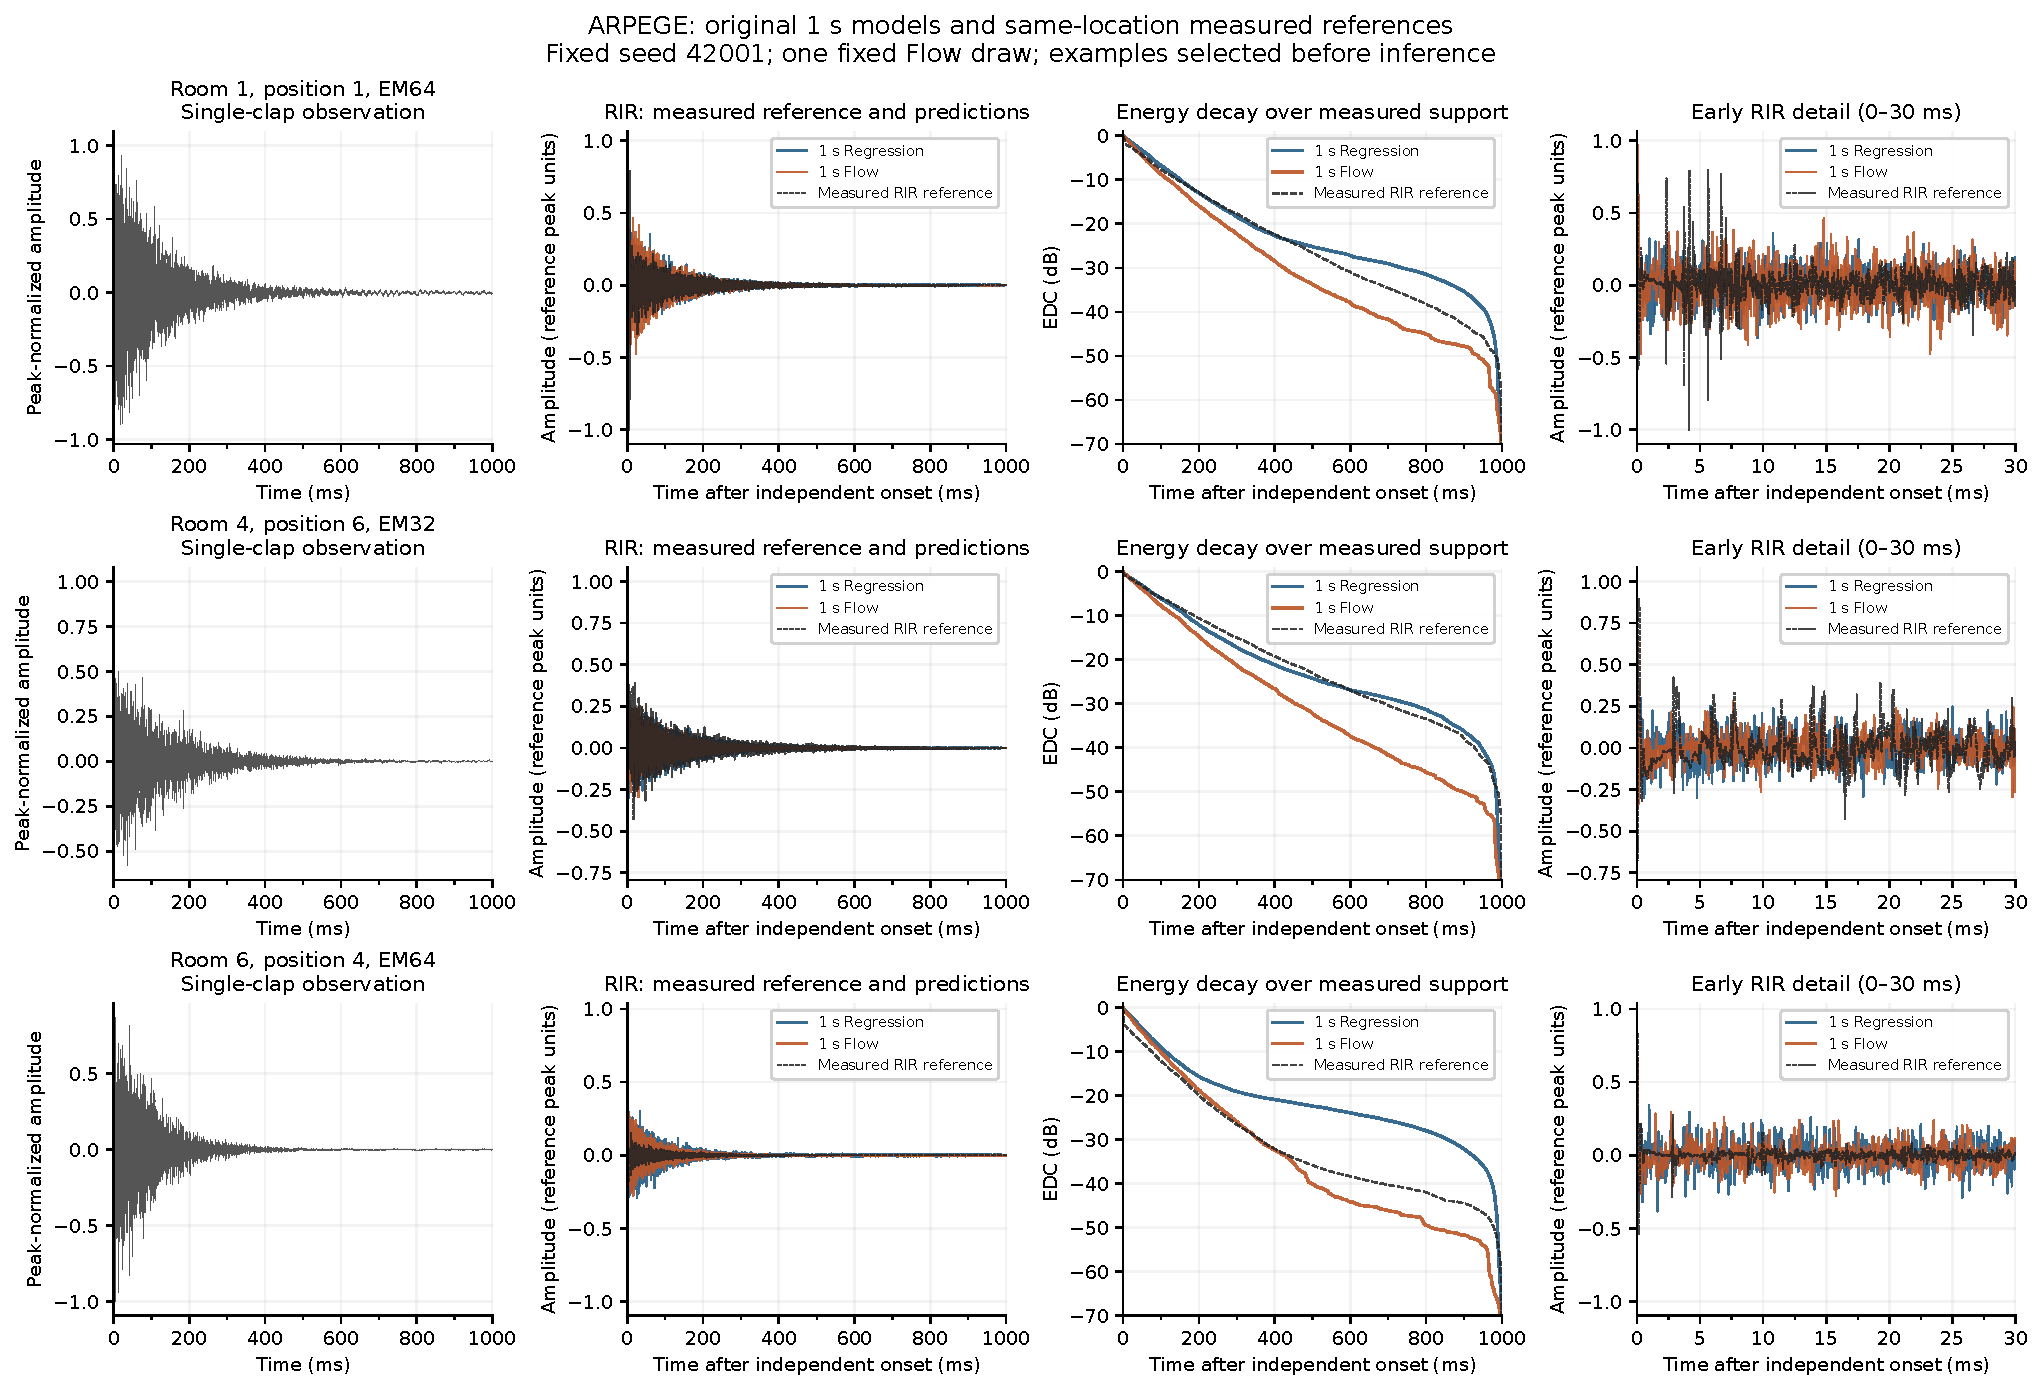
\includegraphics[width=\linewidth]{figures/arpege_examples.pdf}
%     \caption{Representative ARPEGE examples from three rooms. From left to
%     right, each row shows the recorded handclap observation, the measured
%     reference RIR with Regression and Flow predictions, the corresponding
%     energy-decay curves, and the first 30 ms of the RIR. Examples are selected
%     from the input metadata before inference. Both models use training seed
%     42001; the stochastic Flow model is shown with one sample. The measured
%     reference is obtained at the same annotated source and receiver geometry,
%     but handclap and loudspeaker directivities are not assumed to match.}
%     \label{fig:arpege-examples}
% \end{figure}

% \begin{figure}[t]
%     \centering
%     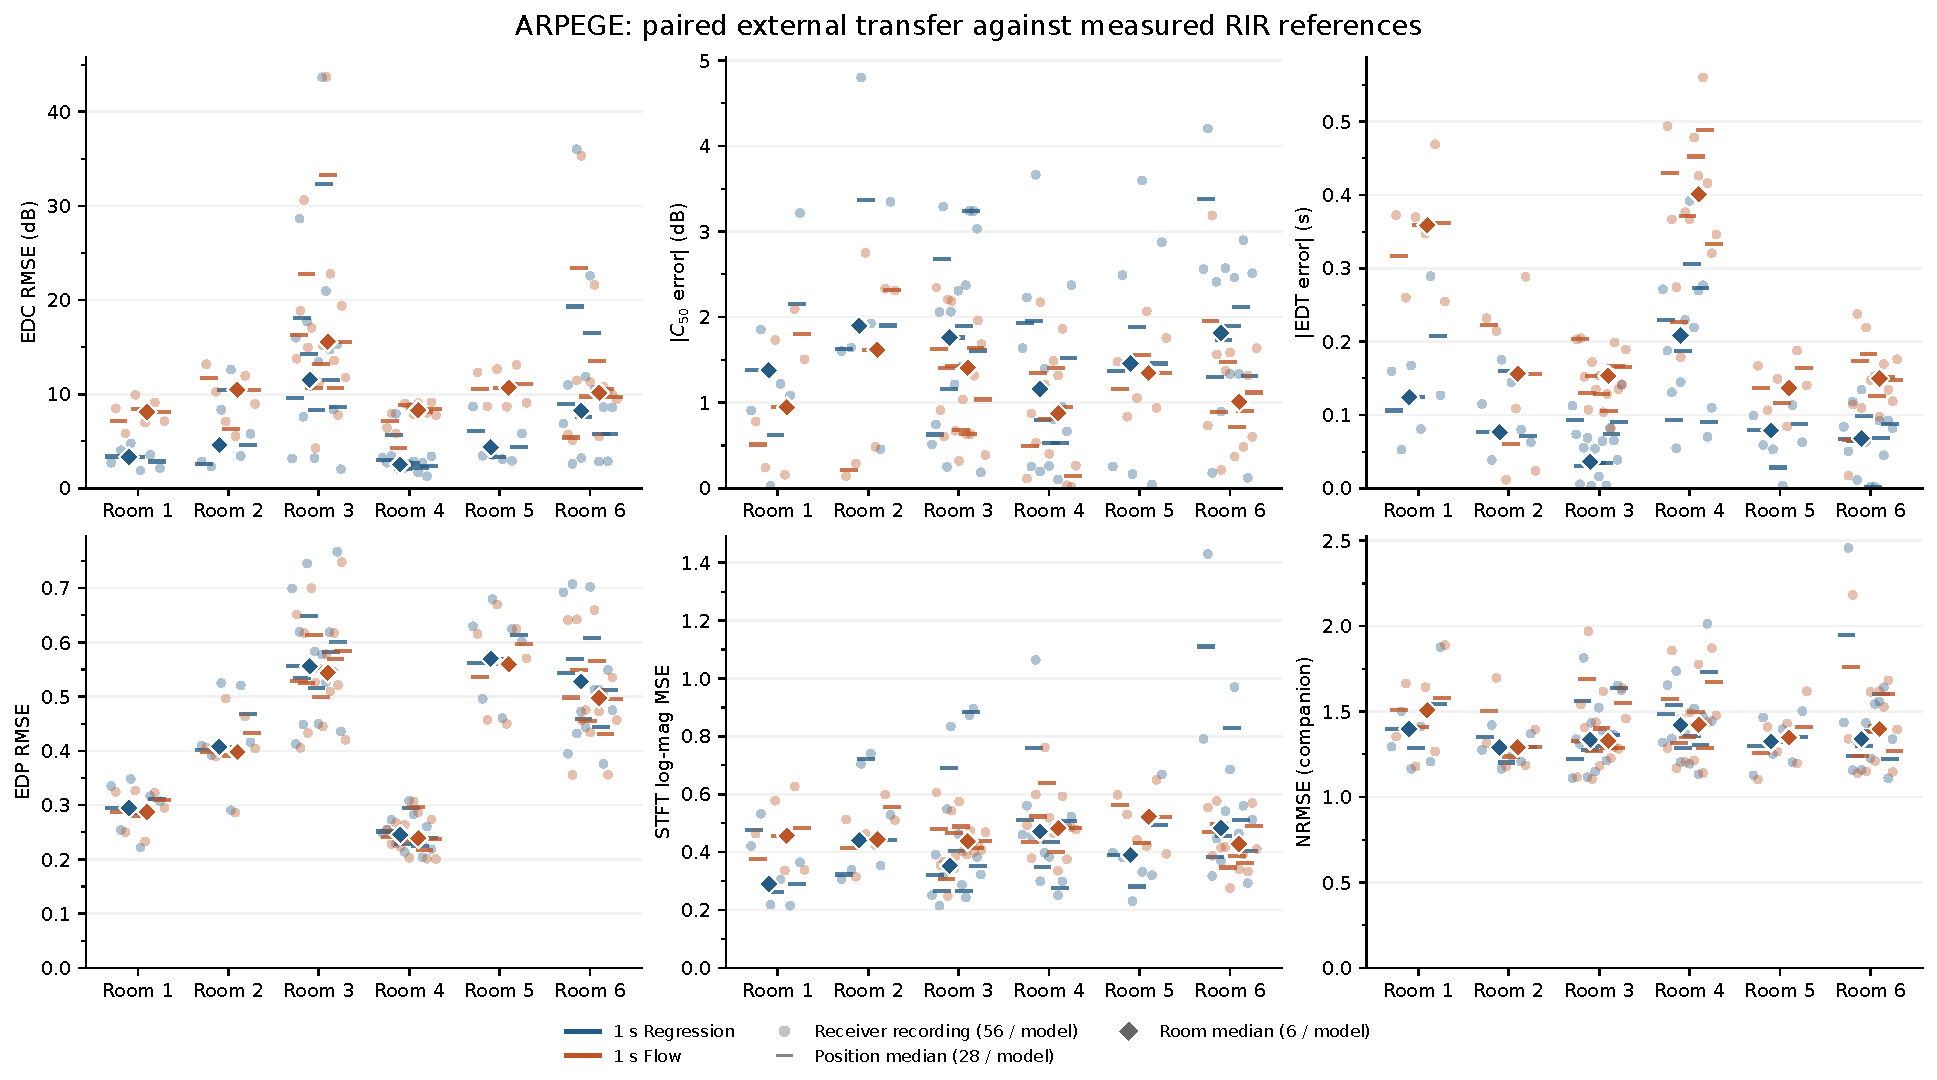
\includegraphics[width=\linewidth]{figures/arpege_external_transfer.pdf}
%     \caption{External paired evaluation on ARPEGE across six rooms.
%     Points denote receiver recordings, short horizontal markers denote
%     position medians, and diamonds denote room medians. Regression and Flow
%     are evaluated against same-location measured reference RIRs using one
%     training seed. The panels report EDC RMSE, absolute $C_{50}$ error,
%     absolute EDT error, EDP RMSE, log-magnitude STFT MSE, and NRMSE.
%     NRMSE is included as a companion metric.}
%     \label{fig:arpege-transfer}
% \end{figure}
% The phone acquisition contains 291 detected acoustic events: 280 protocol
% handclaps, seven additional handclaps, three handling events, and one environmental
% event. The analysis uses the 280 protocol handclaps, comprising seven rooms,
% eight handclap modes, and five recordings per mode. Segments are decoded from the
% original 48-kHz mono M4A recordings, resampled to 44.1 kHz, aligned using the recorded
% onset pre-pad, and converted to float32. No amplitude normalization,
% high-pass filtering, or denoising is applied, so ambient recording noise is
% retained.
% For qualitative figures and audio examples, one unclipped protocol handclap per
% room--mode cell is selected using a prediction-independent pre-handclap-SNR rule,
% giving 56 examples. The consistency analysis uses all 280 protocol handclaps.

% For descriptor $d$, let $d_{rmk}$ denote the median prediction across training
% seeds for physical clap $k$, mode $m$, and room $r$. We define
% \begin{equation}
%  c_r=\mathrm{median}_{m,k}d_{rmk},\qquad
%  H_{rm}=\mathrm{median}_{k}|d_{rmk}-c_r|.
%  \label{eq:consistency}
% \end{equation}
% Here $c_r$ is the room-wise center of the predictions, not a reference RIR.
% Repeatability is also summarized using the five-clap interquartile range (IQR)
% within each room--mode cell, followed by medians across modes and rooms. The
% result is \EsixC{} dB for $C_{50}$ and \EsixEDT{} s for EDT.

% Figure~\ref{fig:phone-consistency} shows the five-clap distributions for all
% room--mode cells. Figure~\ref{fig:phone-edc} shows predicted EDCs for selected
% examples. Because no paired reference RIR exists, these results quantify
% repeatability and sensitivity to clap mode, not reconstruction accuracy. The
% model was trained without added background noise, so the observed deployment
% variation cannot be attributed specifically to noise.

% We additionally recorded handclaps with an iPhone 15 in seven rooms using eight handclap modes and five repetitions per mode. The recordings are decoded
% at 48 kHz and resampled to 44.1 kHz without denoising. To illustrate real-world behavior, we select a medium-size meeting room and an acoustics hallway based on room metadata before inference. For each room and handclap mode, we choose the unclipped recording with the highest pre-handclap SNR using only the input recording. The same one-second Regression model is applied to
% all selected recordings.

We recorded 280 protocol handclaps with an iPhone 15 in seven rooms, comprising
eight handclap modes and five repetitions per mode. Recordings are decoded at
48~kHz, resampled to 44.1~kHz, aligned using the recorded onset pre-pad, and
used without amplitude normalization, high-pass filtering, or denoising. For
each room and handclap mode, one unclipped recording with the highest
pre-handclap SNR is selected using only the input recording before inference;
Fig.~\ref{fig:phone-spectrum} shows examples from a medium-size meeting room
and a highly reverberant hallway with the same one-second regressor.

Figure~\ref{fig:phone-spectrum} compares phone-recorded handclaps with their
inferred RIRs in the spectral and time domains. The upper panels show
1/12-octave-averaged spectra over 0.1--15~kHz using a common 0--0.9-s
interval. Each spectrum is normalized to its own mean FFT-bin power over
0.1--10~kHz. The lower panels show RMS level over the first 250~ms on the
original digital scale (dBFS), without per-signal normalization.
The recorded spectra show substantial mode-dependent variation in both rooms,
while the inferred spectra are visibly more consistent across modes. The RMS
envelopes likewise show similar decay behavior across the inferred responses
within each room. These observations suggest reduced sensitivity to
clap-specific spectral characteristics; however, because no paired reference
RIR is available, they do not establish real-world reconstruction accuracy.





%\begin{figure}[t]
%    \centering
%    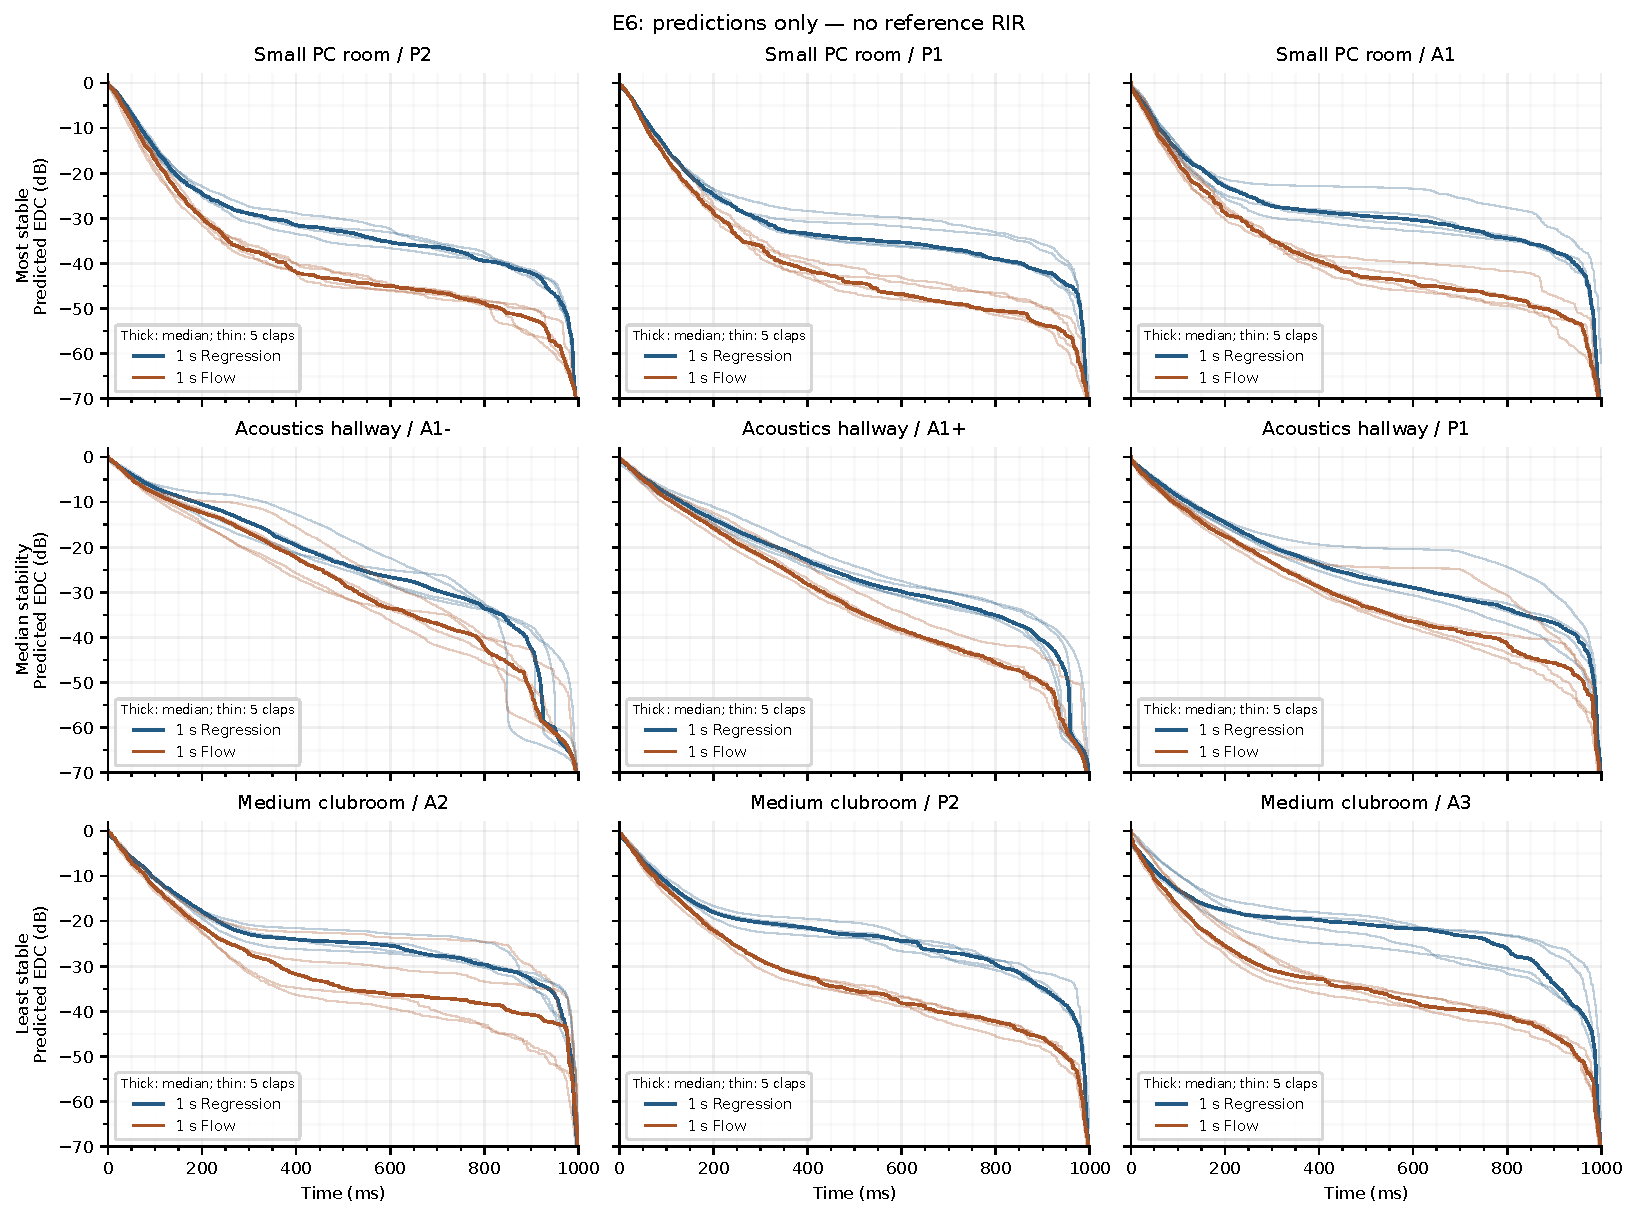
\includegraphics[width=\linewidth]{figures/e6_phone_examples.pdf}
%    \caption{Prediction-only EDC overlays for phone recordings from rooms with
%    low, median, and high $C_{50}$ mode dispersion. Within each room, the three
%    displayed modes span low, intermediate, and high median predicted
%    $C_{50}$. Thin curves show the five recorded claps and thick curves show
%    the median across those five claps for each model. Regression and flow matching use seed 42001; the Flow curves
%    use one sample per input. No reference RIR is available.}
%    \label{fig:phone-edc}
%\end{figure}

% \begin{figure}[t]
%     \centering
%     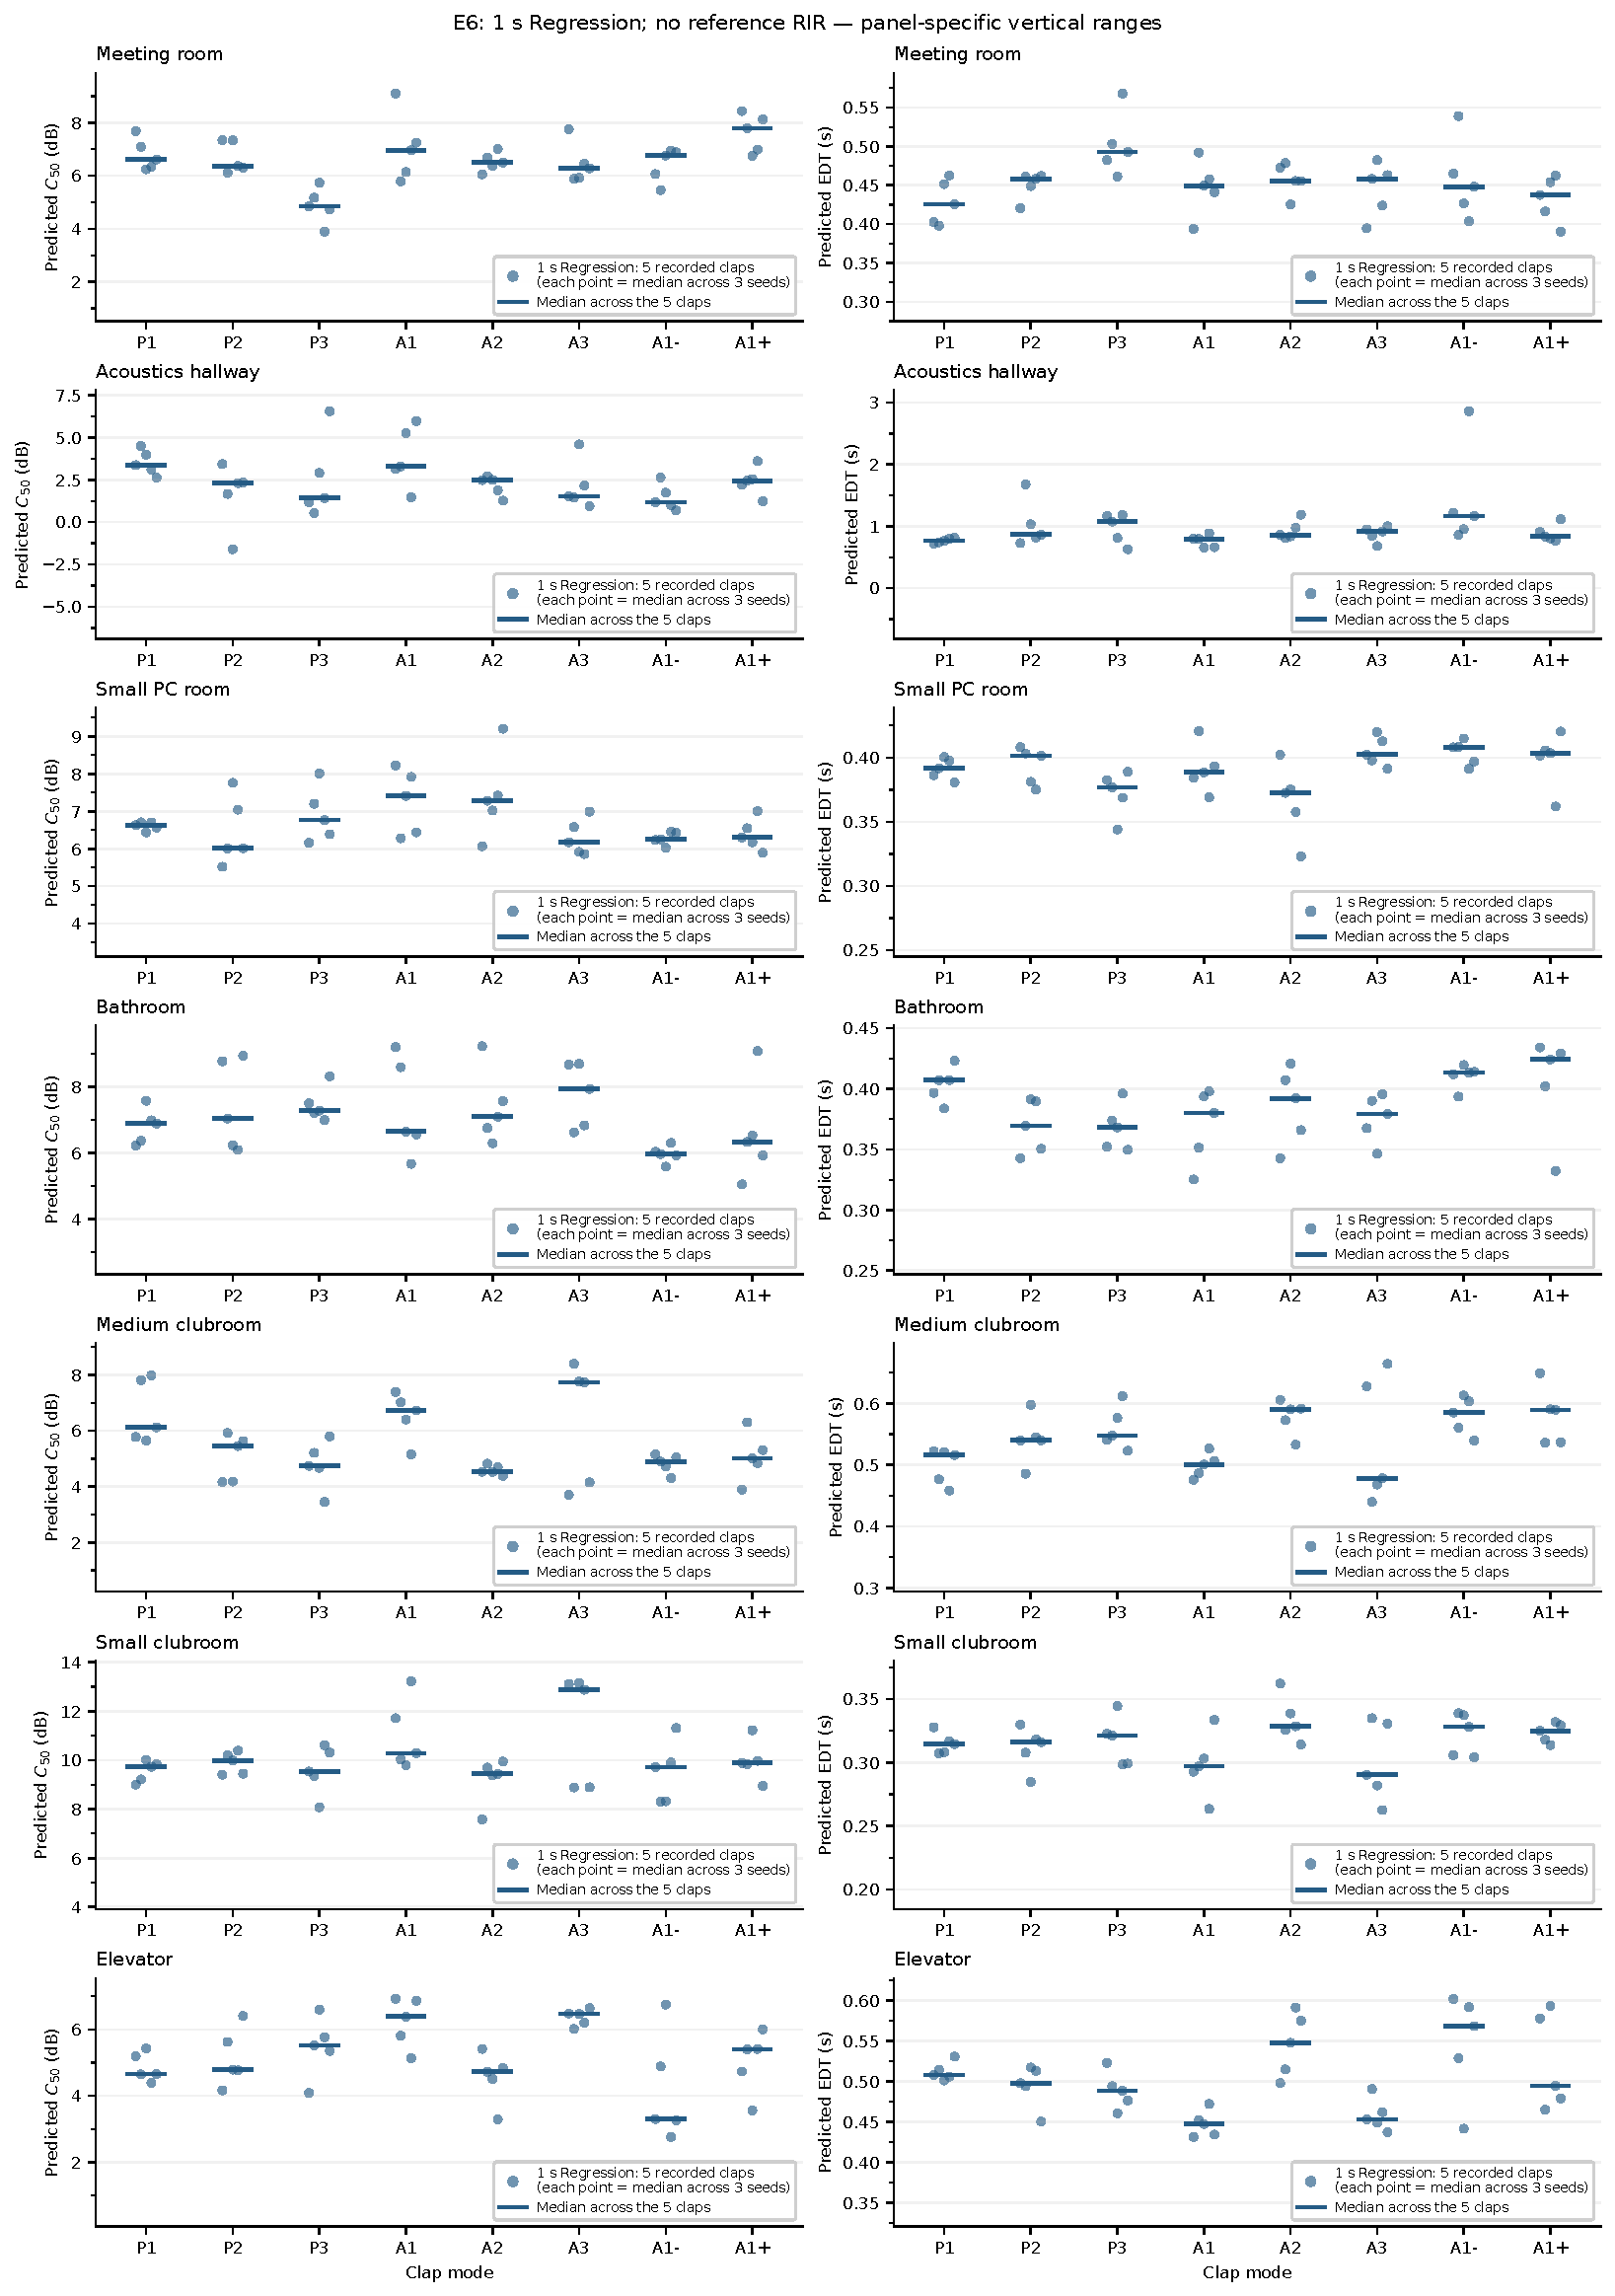
\includegraphics[width=\linewidth]{figures/e6_phone_consistency.pdf}
%     \caption{Phone-recording prediction consistency across seven rooms and
%     eight clap modes. Each point represents one of five protocol claps and is
%     summarized across the three Regression training seeds; horizontal markers
%     show the within-mode median. The panels report predicted $C_{50}$ and EDT,
%     not reconstruction error, because the recordings have no paired reference
%     RIR.}
%     \label{fig:phone-consistency}
% \end{figure}

% \begin{figure}[t]
%     \centering
%     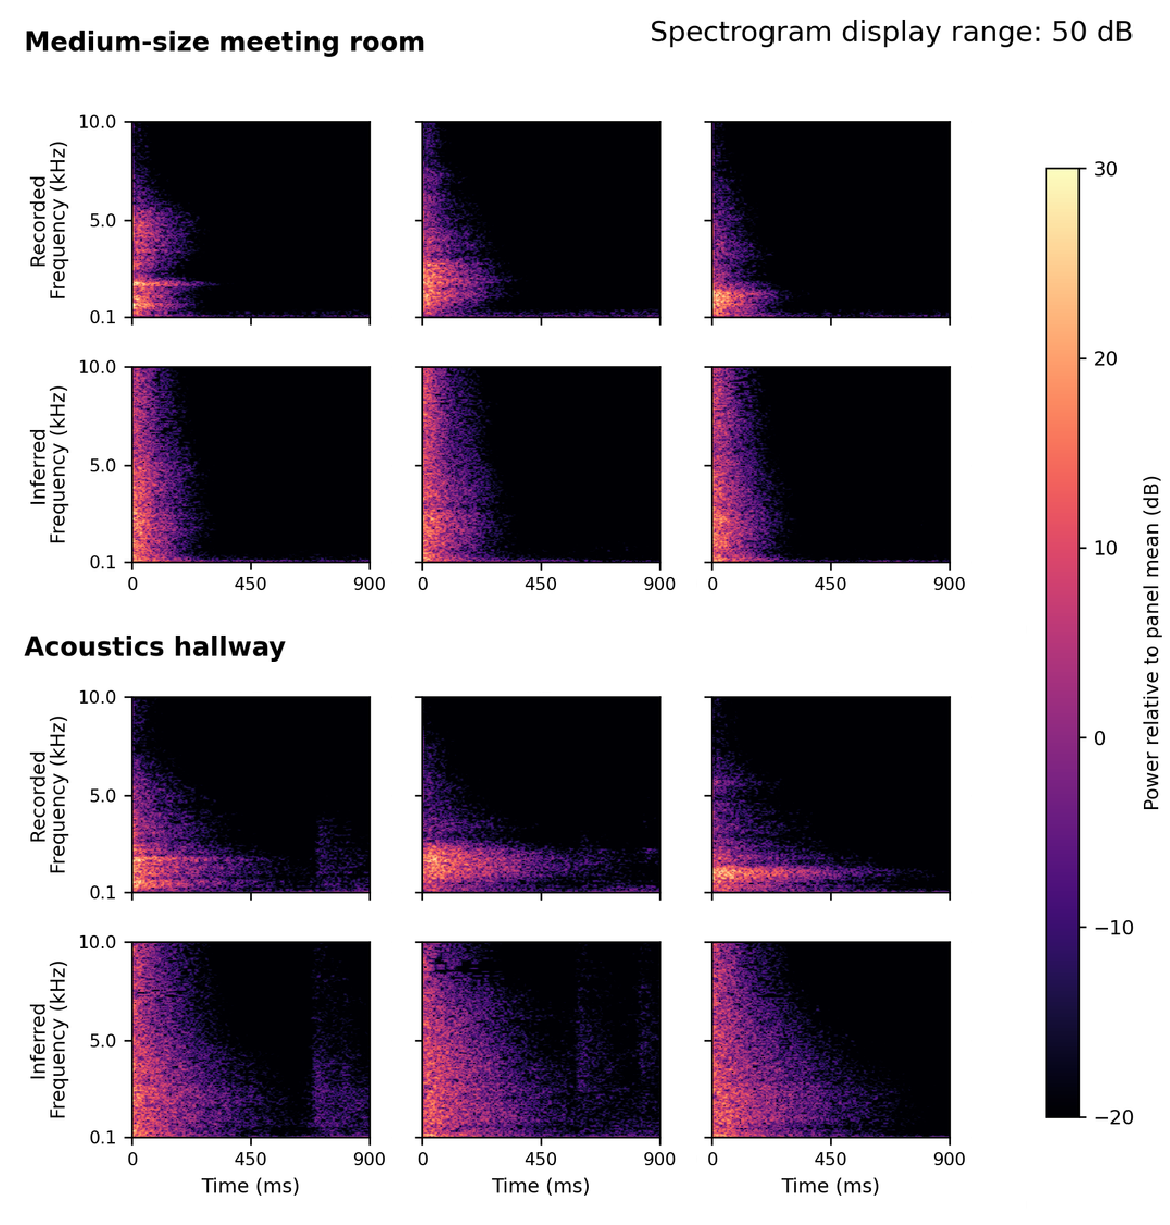
\includegraphics[width=\linewidth]{figures/phone_spectrogram_range_50db_3examples_column.pdf}
%     \vspace{-0.5cm}
%    \caption{Spectrograms of eight handclap modes
% (\cite{repp1987sound,peltola2007synthesis}; three shown here) in a
% meeting room (top) and acoustics hallway (bottom), with recordings above
% their inferred RIRs. One unclipped sample per room and mode is selected by
% input-only pre-handclap SNR. Panels span 0--0.9 s and 0.1--10 kHz, with
% per-panel mean-power normalization and shared $-20$ to $+30$ dB limits.
% No paired reference RIR is available.}
%     \label{fig:phone-qualitative}
%     \vspace{-0.5cm}
% \end{figure}

\begin{figure}[t]
    \centering
   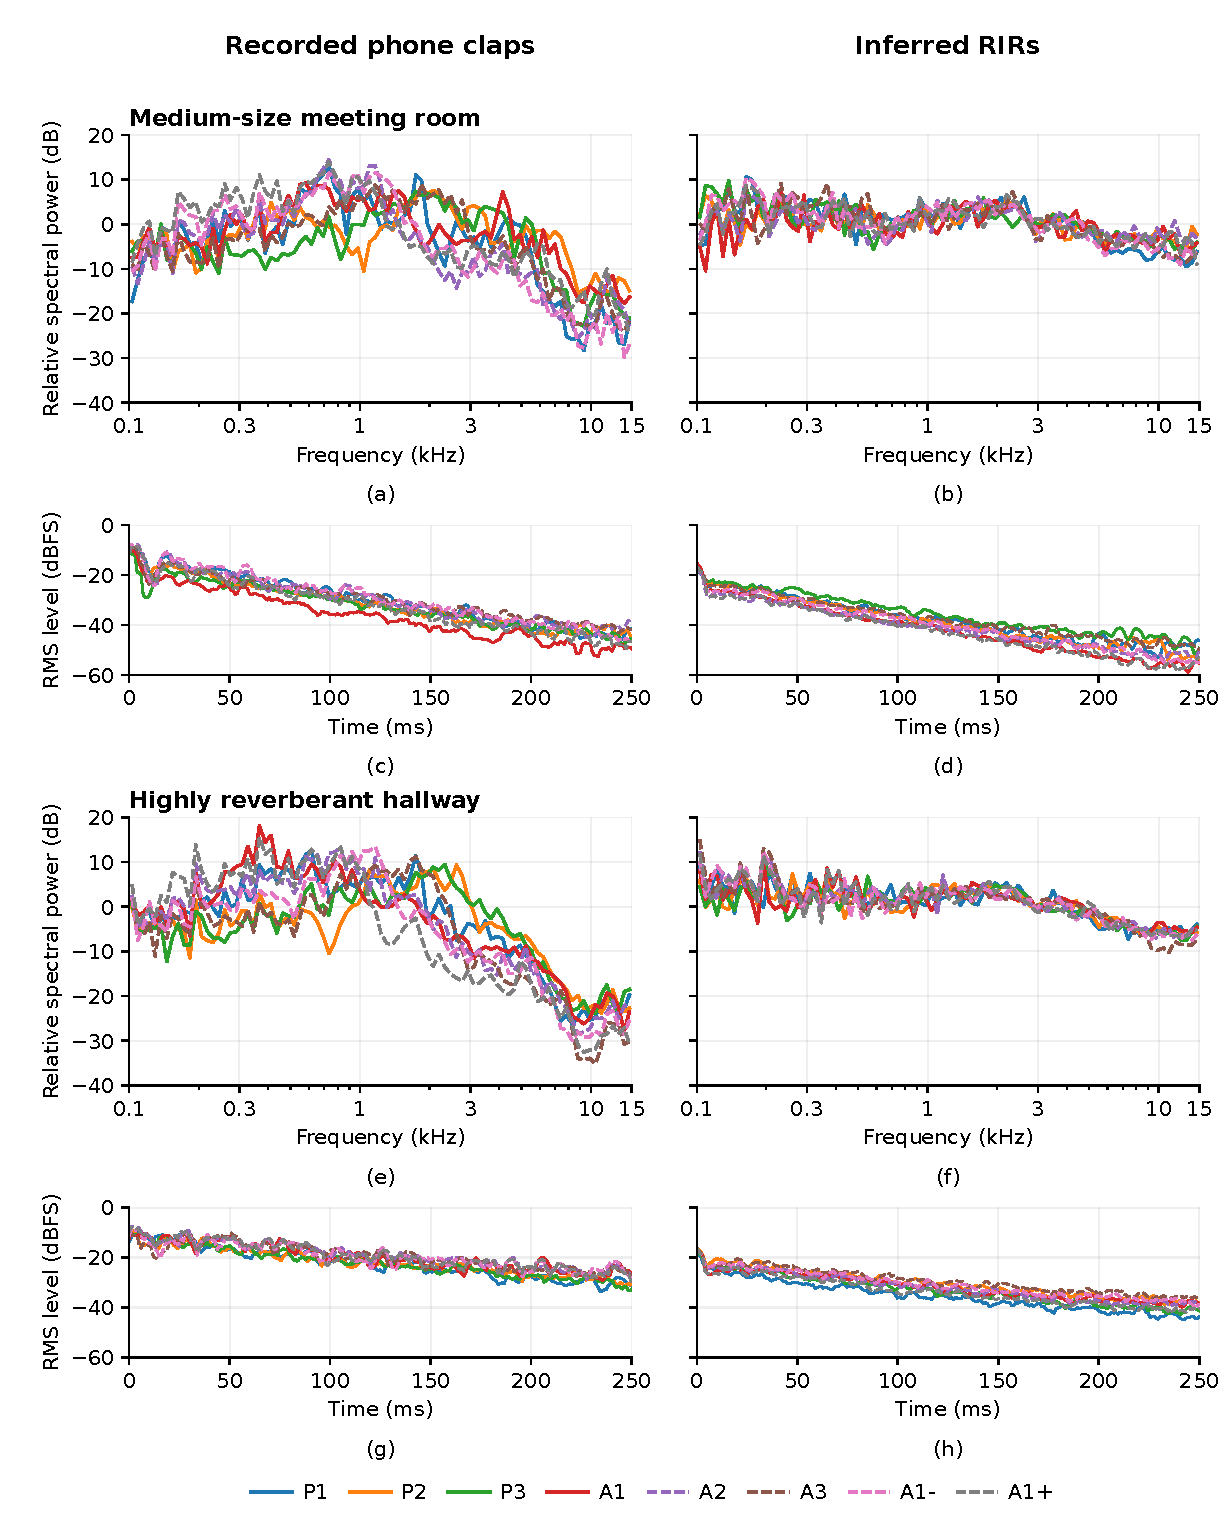
\includegraphics[width=\columnwidth]
    {figures/phone_qualitative_spectrum_time.pdf}
    \vspace{-0.7cm}
\caption{Phone-recorded handclaps (left) and corresponding Regression RIR
estimates (right) for eight handclap modes in a medium-size meeting room and
a highly reverberant hallway. For each room, the upper panels show spectra
and the lower panels show RMS envelopes.}
\label{fig:phone-spectrum}
    \vspace{-0.5cm}
\end{figure}





\section{Conclusion}
\label{sec:conclusion}

% \vesa{Let's first summarize briefly what this paper was about. Limitations may also be mentioned, but only what has been described elsewhere in the paper - no new info anymore. [Done]}

% We studied estimation of a one-second room impulse response from a single
% handclap and introduced an anechoic corpus of 2,588 handclaps from 17
% participants. Known-excitation inversion shows that the RIR is recoverable
% when the handclap waveform is available, while using the first 3 ms of the
% reverberant recording as an excitation estimate gives substantially larger
% errors. A two-stage time--frequency/time-domain Regression model improves on
% this 3-ms baseline across all reported reconstruction metrics.
% The controlled benchmark is limited by the available reference support,
% including the 92.88-ms Shoebox targets. The phone recordings have no paired
% reference RIR and are therefore evaluated qualitatively. Across the eight handclap
% modes shown, the inferred RIR spectra are more consistent than the recorded
% handclap spectra over much of the analyzed frequency range.

We studied one-second RIR estimation from a single handclap and introduced an
anechoic handclap corpus. Direct regression improves on cropped-excitation
deconvolution while remaining less accurate than known-excitation
deconvolution. Phone-recorded examples qualitatively show reduced
clap-dependent spectral variation, although no paired reference RIR is
available.

\section{Acknowledgments}
This study was conducted when the first author visited the Aalto Acoustics Lab in Jul.--Sept. 2026. This work was supported by the HUCE infrastructure of the Aalto School of Electrical Engineering, the National Science and Technology Council (NSTC), Taiwan (under NTSC 114-2221-E-002-218-MY3, and 114-2218-E-002-006), and National Taiwan University (114L900902 and 115L8909) funded through the Ministry of Education (MOE), Taiwan.


\bibliographystyle{IEEEbib}
\bibliography{2026_claps}



% \cite{}\section{Blind Deconvolution: Formulation and Methods}
% \label{app:blind-method}

% \paragraph{Task.}
% As a supplementary experiment, we study joint recovery of a dry handclap
% excitation $x$ and a room impulse response (RIR) $h$ from a single reverberant
% observation $y$. This differs from the main-paper estimator, which predicts
% only $h$. Both Joint Regression and Joint Flow receive the same single-channel
% observation and estimate the pair $(x,h)$ without access to the reference
% excitation at inference. Signals are sampled at 44.1~kHz; $x$ has 2,205
% samples (50~ms), and $h$ and $y$ have 44,100 samples (1~s). The forward model is
% \begin{equation}
%     y = M_y \odot \mathcal{C}(x,h), \qquad
%     \mathcal{C}(x,h) = (x*h)[0:N_y],
%     \label{eq:blind-forward}
% \end{equation}
% where $*$ is causal linear convolution and $M_y$ excludes unavailable
% reference support. Unknown RIR tails are masked rather than treated as silence.

% Blind decomposition has a scale ambiguity: $(ax,h/a)$ gives the same
% convolution for any nonzero $a$. We therefore fix a canonical digital gain.
% For an aligned dry-clap crop $c$ with signed peak $g$,
% \begin{equation}
%     x=c/g,\qquad h=g\,h_0,
%     \label{eq:blind-gauge}
% \end{equation}
% which preserves $x*h=c*h_0$. Predictions are put into the same pair-preserving
% gauge using the signed peak of $\widehat{x}$. No reference-fitted gain or delay
% is used. Excitation recovery, RIR recovery, and forward consistency are
% reported separately because an accurate product does not guarantee accurate
% individual factors.

% \paragraph{Models.}
% Both joint models use the same hybrid time--frequency/time-domain design with a
% shared observation pathway and separate excitation and RIR outputs. Joint
% Regression predicts $(\widehat{x},\widehat{h})$ directly in one forward pass.
% Joint Flow instead models a time-dependent joint state for $(x,h)$ conditioned
% on $y$ and is initialized independently; it does not use a Regression
% checkpoint, residual anchor, or oracle factor.

% Training uses fixed RMS scales estimated from the training split and reused
% unchanged at validation and external evaluation. For normalized factor
% $q\in\{x,h\}$, Joint Flow uses the straight bridge
% \begin{equation}
%     z_{q,t}=tq+(1-t)\epsilon_q,\qquad
%     v_q^\star=q-\epsilon_q,
%     \label{eq:blind-flow-bridge}
% \end{equation}
% with $t\sim\mathcal{U}(0,1)$ and independent Gaussian noise for the two
% factors.

% Both models receive direct supervision on the true excitation and true RIR,
% not only on their convolution. Let $L_{\mathrm{factor}}$ denote the balanced
% waveform, magnitude, and complex-STFT endpoint losses for $x$ and $h$, and let
% $L_{\mathrm{conv}}$ combine waveform and complex-STFT error between
% $\widehat{x}*\widehat{h}$ and $y$. The frozen objectives are summarized as
% \begin{align}
%     L_{\mathrm{Reg}}
%     &= L_{\mathrm{factor}} + 0.25\,L_{\mathrm{conv}}, \\
%     L_{\mathrm{Flow}}
%     &= L_{\mathrm{FM}} + L_{\mathrm{factor}} + 0.25\,L_{\mathrm{conv}},
%     \label{eq:blind-objectives}
% \end{align}
% where $L_{\mathrm{FM}}$ is the balanced excitation/RIR flow-matching loss.
% Thus, mixed RIR recovery cannot be explained simply by the absence of
% factor-specific supervision.

% \paragraph{Training and inference.}
% The models were trained from scratch for a fixed 20,000 AdamW updates on 872
% pairs from 207 rooms; development used 256 pairs from 62 room-disjoint units.
% The terminal 20,000-update checkpoints were fixed in advance. Regression uses
% one forward pass. Flow uses one fixed draw ($K=1$, inference seed 61002) with
% the frozen 20-NFE sampler, churn 0.5, and no peak projection. No checkpoint,
% seed, draw, or best-of-$K$ selection is performed.

% \section{Prospective External Blind Evaluation}
% \label{app:blind-experiments}

% \paragraph{External benchmark.}
% To test whether the development behavior transfers beyond the training
% providers, we froze both 20,000-update models and constructed a prospective
% external benchmark by convolving held-out dry handclaps with measured ARPEGE
% RIRs. Both factors are therefore known. ARPEGE recorded handclaps are not used
% because no paired dry excitation reference is available for them.

% The final cohort contains 32 measured RIRs from 16 source/receiver geometries
% in four ARPEGE rooms (1, 2, 3, and 5), with EM32 and EM64 receiver
% configurations. A fixed mono convention (physical capsule 0) is used. Each
% geometry is paired with four deterministically selected held-out dry claps
% from participants P08, P15, and P17, all participant- and instance-disjoint
% from joint training and validation. This gives 128 examples per model.
% Membership and preprocessing were fixed before inference. No model,
% checkpoint, threshold, draw, or example selection was changed after seeing
% the results.

% Metrics are organized into three scoreboards:
% (i) excitation-factor recovery (NRMSE, log-magnitude MSE, complex-STFT MSE);
% (ii) RIR-factor recovery (NRMSE, EDC RMSE, absolute $C_{50}$ error, absolute
% EDT error, echo-density-profile RMSE, log-magnitude MSE, complex-STFT MSE);
% and (iii) forward-convolution consistency (NRMSE, waveform MSE,
% complex-STFT MSE). All metrics use valid measured support. Aggregation is by
% median over the four claps for each RIR, receiver RIRs within geometry,
% geometries within room, and finally the four rooms. The repeated claps and RIRs
% are not treated as independent rooms.

% \begin{table}[t]
% \centering
% \small
% \setlength{\tabcolsep}{4pt}
% \caption{Prospective external blind benchmark. Values are medians of four ARPEGE room summaries; the last column counts rooms where Flow has lower error. Lower is better.}
% \label{tab:blind-external}
% \resizebox{\columnwidth}{!}{%
% \begin{tabular}{lrrr}
% \toprule
% Metric & Regression & Flow & Flow-lower rooms \\
% \midrule
% \multicolumn{4}{l}{\textit{A. Excitation-factor recovery}} \\
% $x$ NRMSE & 1.2912 & 1.2727 & 3/4 \\
% $x$ log-mag MSE & 0.5734 & 0.18643 & 4/4 \\
% $x$ complex-STFT MSE & 0.0091944 & 0.0073461 & 4/4 \\
% \addlinespace
% \multicolumn{4}{l}{\textit{B. RIR-factor recovery}} \\
% $h$ NRMSE & 1.0563 & 1.0737 & 2/4 \\
% EDC RMSE (dB) & 6.7663 & 7.0814 & 2/4 \\
% $|\Delta C_{50}|$ (dB) & 2.0026 & 2.1106 & 2/4 \\
% $|\Delta\mathrm{EDT}|$ (s) & 0.16746 & 0.21658 & 2/4 \\
% EDP RMSE & 0.54975 & 0.5337 & 4/4 \\
% $h$ log-mag MSE & 0.31642 & 0.38777 & 0/4 \\
% $h$ complex-STFT MSE & $2.1044\times10^{-6}$ & $2.3337\times10^{-6}$ & 0/4 \\
% \addlinespace
% \multicolumn{4}{l}{\textit{C. Forward-convolution consistency}} \\
% $x*h$ NRMSE & 0.93933 & 0.86010 & 4/4 \\
% $x*h$ waveform MSE & 0.00016926 & 0.00014419 & 4/4 \\
% $x*h$ complex-STFT MSE & 0.00015017 & 0.00013808 & 4/4 \\
% \bottomrule
% \end{tabular}%
% }
% \end{table}

% \paragraph{Results.}
% On the prospective ARPEGE benchmark, Flow transfers its advantage in
% excitation spectral recovery and forward consistency. Excitation log-magnitude
% MSE decreases from 0.5734 to 0.1864 (67.5\%), while excitation complex-STFT
% MSE decreases by 20.1\%; both improve in all four rooms. Excitation NRMSE
% changes only modestly, from 1.2912 to 1.2727. All three forward-consistency
% metrics favor Flow in all four rooms, with convolution NRMSE decreasing from
% 0.9393 to 0.8601 (8.4\%).

% True RIR recovery does not show the same transfer. Flow is slightly worse in
% RIR NRMSE (1.0737 vs.\ 1.0563) and generally worse in EDC, $C_{50}$, EDT, and
% RIR spectral errors; EDP is the exception. Thus, the joint Flow model better
% recovers aspects of the excitation and more accurately reconstructs the
% observed reverberant signal, but it does not recover the true RIR more
% accurately overall.

% \begin{figure}[t]
%     \centering
%     \includegraphics[width=\columnwidth]
%     {figures/arpege_blind_external_examples.pdf}
%     \caption{Representative examples from four ARPEGE rooms. Columns show the known dry excitation, measured RIR, valid-support EDC, and observed versus reconstructed reverberant clap. Example membership was fixed before inference; no reference-fitted gain or delay is used.}
%     \label{fig:blind-external-examples}
% \end{figure}

% \paragraph{Interpretation and limits.}
% The external benchmark supports partial transfer of Flow's excitation-spectrum
% and forward-consistency advantages, but not a general advantage in recovery of
% the true RIR factor. Better reconstruction of $x*h$ therefore does not by
% itself establish correct recovery of the individual factors. These results do
% not identify whether the remaining error is caused by factor ambiguity,
% architecture, optimization, or another mechanism. The comparison uses one
% training seed, one Flow draw, single-channel observations, finite RIR support,
% and only four external rooms, so it should be interpreted as supplementary
% development evidence rather than a claim that blind deconvolution is solved.



% \section{Paired Regression--Flow Uncertainty}
% \label{app:paired}

% For MIT and OpenAIR, we estimate room-level paired
% Flow-minus-Regression differences. Positive values indicate larger error for
% flow matching and therefore favor regression. Confidence intervals are
% obtained by resampling rooms. Providers with too few independent rooms for
% this analysis are reported descriptively in the main text.

% \begin{table}[t]
% \centering
% \caption{Paired room-level Flow-minus-Regression median differences with 95\%
% room-cluster confidence intervals. Positive values favor regression. MIT has
% 42 rooms and OpenAIR has nine.}
% \label{tab:paired-comparison}
% \resizebox{\columnwidth}{!}{%
% \begin{tabular}{llr@{\ }l}
% \toprule
% Provider & Metric & \multicolumn{2}{c}{Difference [95\% CI]} \\
% \midrule
% MIT & EDC RMSE (dB) & +3.225879 & [+1.985177, +5.126741] \\
% MIT & $|\Delta C_{50}|$ (dB) & +1.605907 & [+1.160338, +1.786019] \\
% MIT & $|\Delta \mathrm{EDT}|$ (s) & +0.000758 & [+0.000047, +0.009082] \\
% MIT & EDP RMSE & +0.015157 & [+0.009565, +0.030817] \\
% MIT & Log-mag MSE & +0.202700 & [+0.121360, +0.264762] \\
% MIT & NRMSE & +0.050167 & [+0.005130, +0.085873] \\
% OpenAIR & EDC RMSE (dB) & +1.818563 & [+0.953841, +3.347828] \\
% OpenAIR & $|\Delta C_{50}|$ (dB) & +0.011028 & [-0.318139, +0.226558] \\
% OpenAIR & $|\Delta \mathrm{EDT}|$ (s) & +0.018226 & [-0.017163, +0.035009] \\
% OpenAIR & EDP RMSE & +0.008728 & [+0.003738, +0.019993] \\
% OpenAIR & Log-mag MSE & +0.221281 & [+0.126458, +0.310222] \\
% OpenAIR & NRMSE & +0.027901 & [-0.061584, +0.084303] \\
% \bottomrule
% \end{tabular}%
% }
% \end{table}

% \section{Flow-Model Diagnostics}
% \label{app:flow}

% For a teacher-path state
% \begin{equation}
%     h_{\tau}=\tau h+(1-\tau)\epsilon,
% \end{equation}
% the implied endpoint estimate satisfies
% \begin{equation}
%     \widehat h_{\tau}-h
%     =(1-\tau)(\widehat v-v^\star),
% \end{equation}
% and hence
% \begin{equation}
%     E_h(\tau)=(1-\tau)^2E_v(\tau),
% \end{equation}
% where $E_v$ is velocity-prediction MSE and $E_h$ is the corresponding
% endpoint MSE. Endpoint error can therefore decrease as $\tau$ approaches one
% without a corresponding reduction in velocity error.

% Figure~\ref{fig:flow-diagnostics} compares teacher-path velocity error,
% endpoint error along the model's sampled trajectory, and state and velocity
% divergence between teacher and sampled trajectories. Stochastic churn also
% perturbs the sampled path, so the divergence terms measure trajectory
% discrepancy rather than pure vector-field error. Across the five providers,
% the own-trajectory endpoint error remains strongly provider dependent.

% \begin{figure}
%     \centering
%     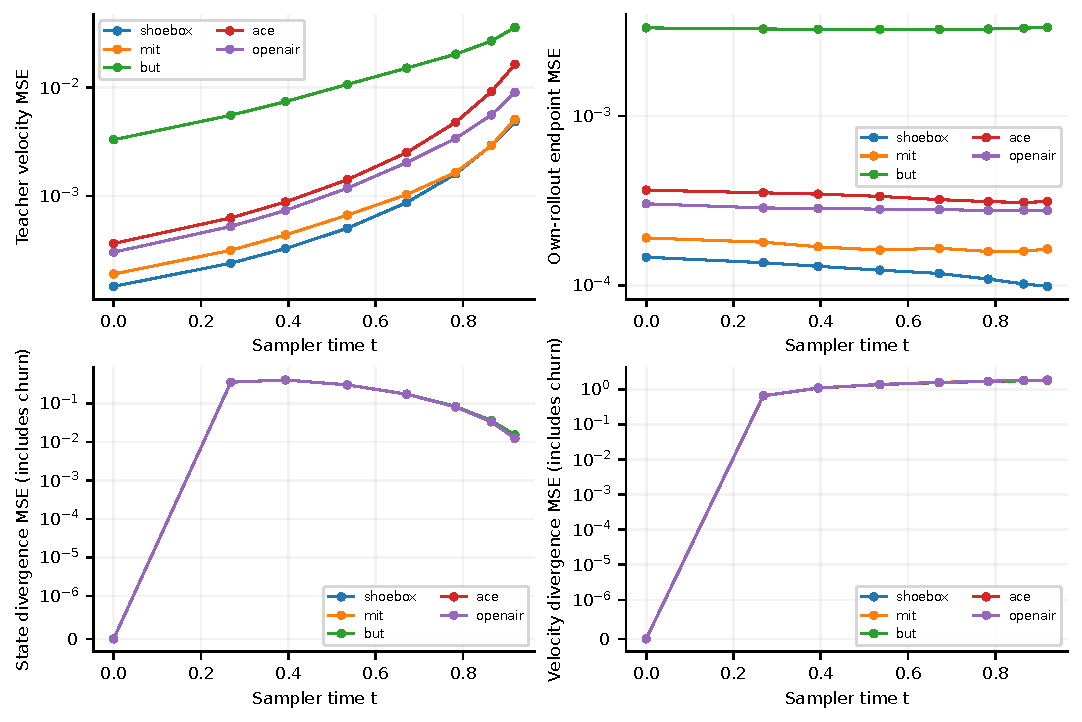
\includegraphics[width=0.9\linewidth]{figures/flow_mechanism_current.pdf}
%     \caption{One-second flow-matching model across sampler
%     time. The panels show teacher-path velocity MSE, endpoint MSE along the
%     sampled trajectory, state divergence, and velocity divergence. State and
%     velocity divergence include the effect of stochastic churn.}
%     \label{fig:flow-diagnostics}
% \end{figure}

% The complex STFT error decomposes as
% \begin{align}
%     |\widehat S-S|^2
%     ={}& (|\widehat S|-|S|)^2 \\
%       &+2|\widehat S||S|
%         \left(1-\cos\Delta\phi\right).
% \end{align}
% The first term is a magnitude error and the second is phase related. In
% Table~\ref{tab:phase}, the phase-related term accounts for more than half of
% the complex-STFT error for every provider. A magnitude-only auxiliary loss
% directly addresses the first term, while waveform-domain velocity supervision
% continues to constrain the full signal.

% \begin{table}
% \centering
% \caption{Complex-STFT error decomposition for the one-second flow model over
% valid RIR support.}
% \label{tab:phase}
% \begin{tabular}{lcc}
% \toprule
% Provider & Magnitude share & Phase-related share \\
% \midrule
% Shoebox & 0.274 & 0.726 \\
% MIT     & 0.445 & 0.555 \\
% BUT     & 0.302 & 0.698 \\
% ACE     & 0.328 & 0.672 \\
% OpenAIR & 0.341 & 0.659 \\
% \bottomrule
% \end{tabular}
% \end{table}

% \section{Additional Phone-Recording Figures}

% The following figures provide additional context for the phone experiment.
% Because no paired reference RIR is available, they characterize prediction
% dispersion and the recorded input conditions rather than reconstruction
% accuracy.

% \begin{figure}
%     \centering
%     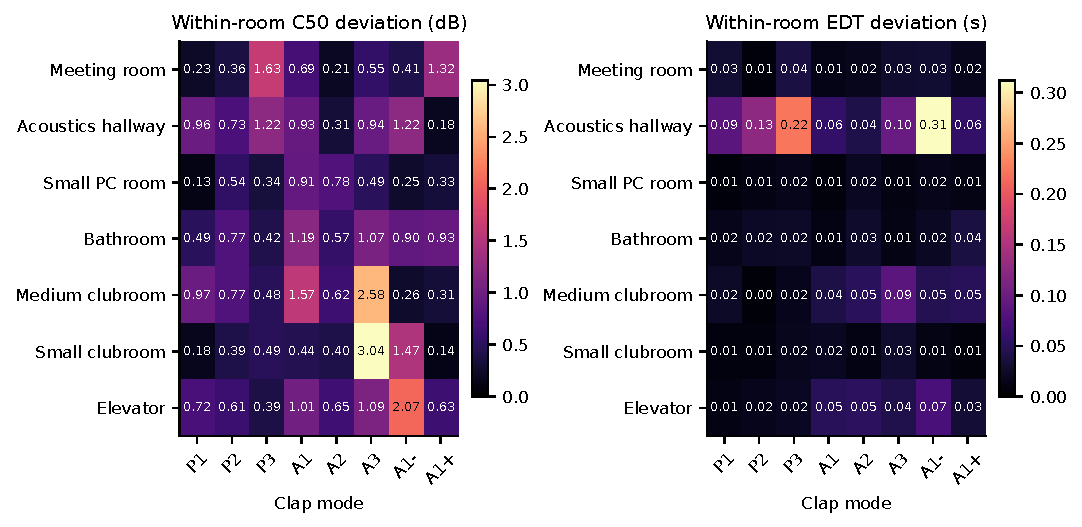
\includegraphics[width=\linewidth]{figures/e6_phone_robustness.pdf}
%     \caption{Within-room prediction dispersion across clap modes. Each cell
%     shows the median absolute descriptor deviation from the room-wise
%     prediction center in Eq.~\eqref{eq:consistency}, in dB for $C_{50}$ and
%     seconds for EDT. Lower values indicate greater within-room consistency.}
%     \label{fig:phone-heatmap}
% \end{figure}

% Figure~\ref{fig:phone-heatmap} summarizes descriptor dispersion across
% room--mode combinations. It should be interpreted together with the five-clap
% distributions in Fig.~\ref{fig:phone-consistency}.

% \begin{figure}
%     \centering
%     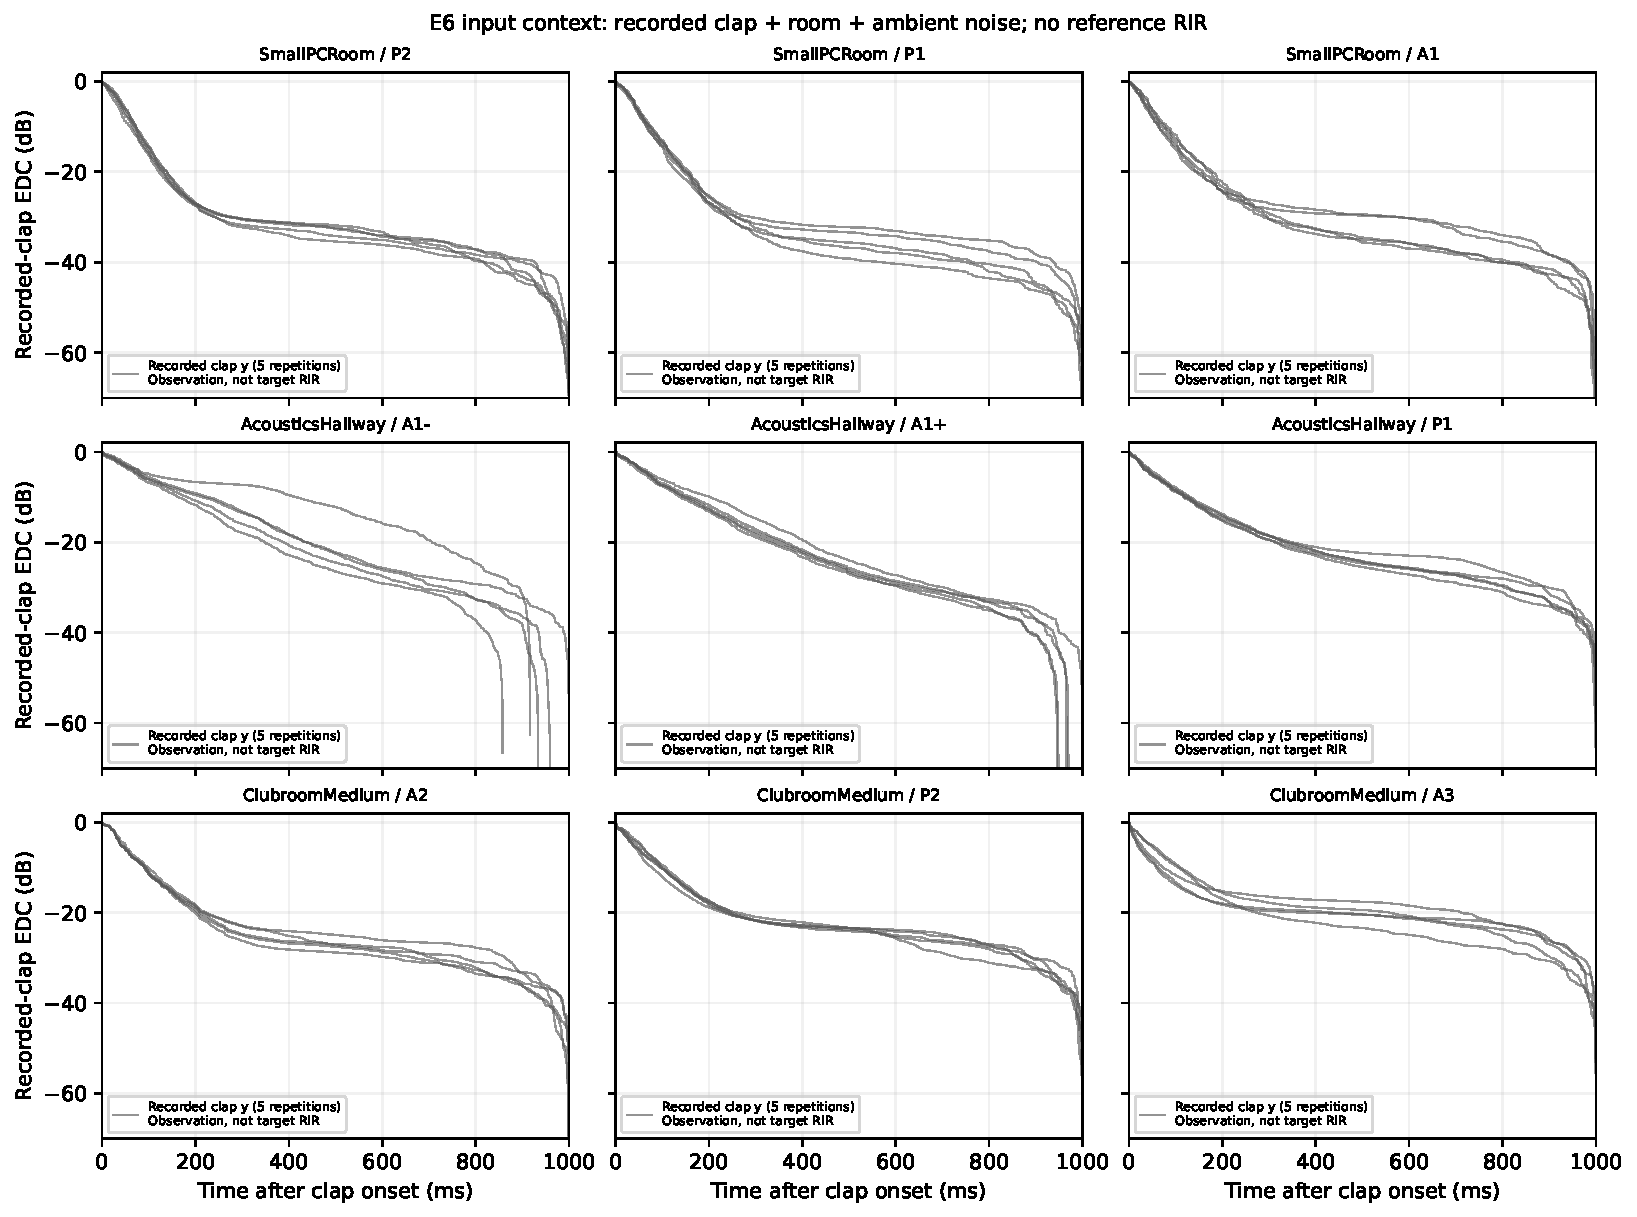
\includegraphics[width=\linewidth]{figures/e6_phone_recording_context.pdf}
%     \caption{Reverse-integrated energy of the recorded phone claps for the same
%     representative room--mode cells as Fig.~\ref{fig:phone-edc}. Each curve
%     includes the handclap excitation, room response, and ambient noise. Curves
%     use at most one second after the recorded onset and stop at the available
%     recording support.}
%     \label{fig:phone-input}
% \end{figure}

% Figure~\ref{fig:phone-input} documents the input recordings associated with
% the qualitative prediction examples. These curves are observations rather
% than reference RIRs and are not used to compute reconstruction error.

\end{document}
